% BLOC-BOT thesis -- main file. Compile with: latexmk -pdf main.tex (uses biber).
\documentclass[12pt,a4paper]{report}

\usepackage[utf8]{inputenc}
\usepackage[T1]{fontenc}
\usepackage{graphicx}
\usepackage{float}
\usepackage{booktabs}
\usepackage{amsmath}
\usepackage[hidelinks]{hyperref}
\usepackage[style=ieee,backend=biber]{biblatex}
\addbibresource{references.bib}

% Figures are read straight from the CAD output folder, so re-rendered images are
% picked up automatically.
\graphicspath{{../CAD/out/}}

\title{BLOC-BOT}
\author{TODO: author}
\date{\today}

\begin{document}
\maketitle
\tableofcontents

\chapter{Motor bracket design}
% Placeholder chapter: shows how to use the figure library and the bibliography.
The motor and sensor dimensions are taken from the reference models
\cite{ttmotor_model,lm393_sensor_model}, and the bracket was modelled in
Autodesk Fusion \cite{fusion360}. Figure~\ref{fig:sensor-side} shows the encoder
disc in the sensor fork.

% Figure library for the thesis. % Figure library for the thesis. % Figure library for the thesis. \input{figures} where needed, or copy single blocks.
% Images live in ../CAD/out/ (see \graphicspath in main.tex), so re-rendering them in
% Fusion updates the thesis without copying files.
% Every figure is also registered in tracking/log.md with how it was produced.
% Naming: label fig:<topic>-<view>.

% F01 -- made with Fusion viewport.saveAsImageFile, iso top-right view, plate hidden
\begin{figure}[htbp]
  \centering
  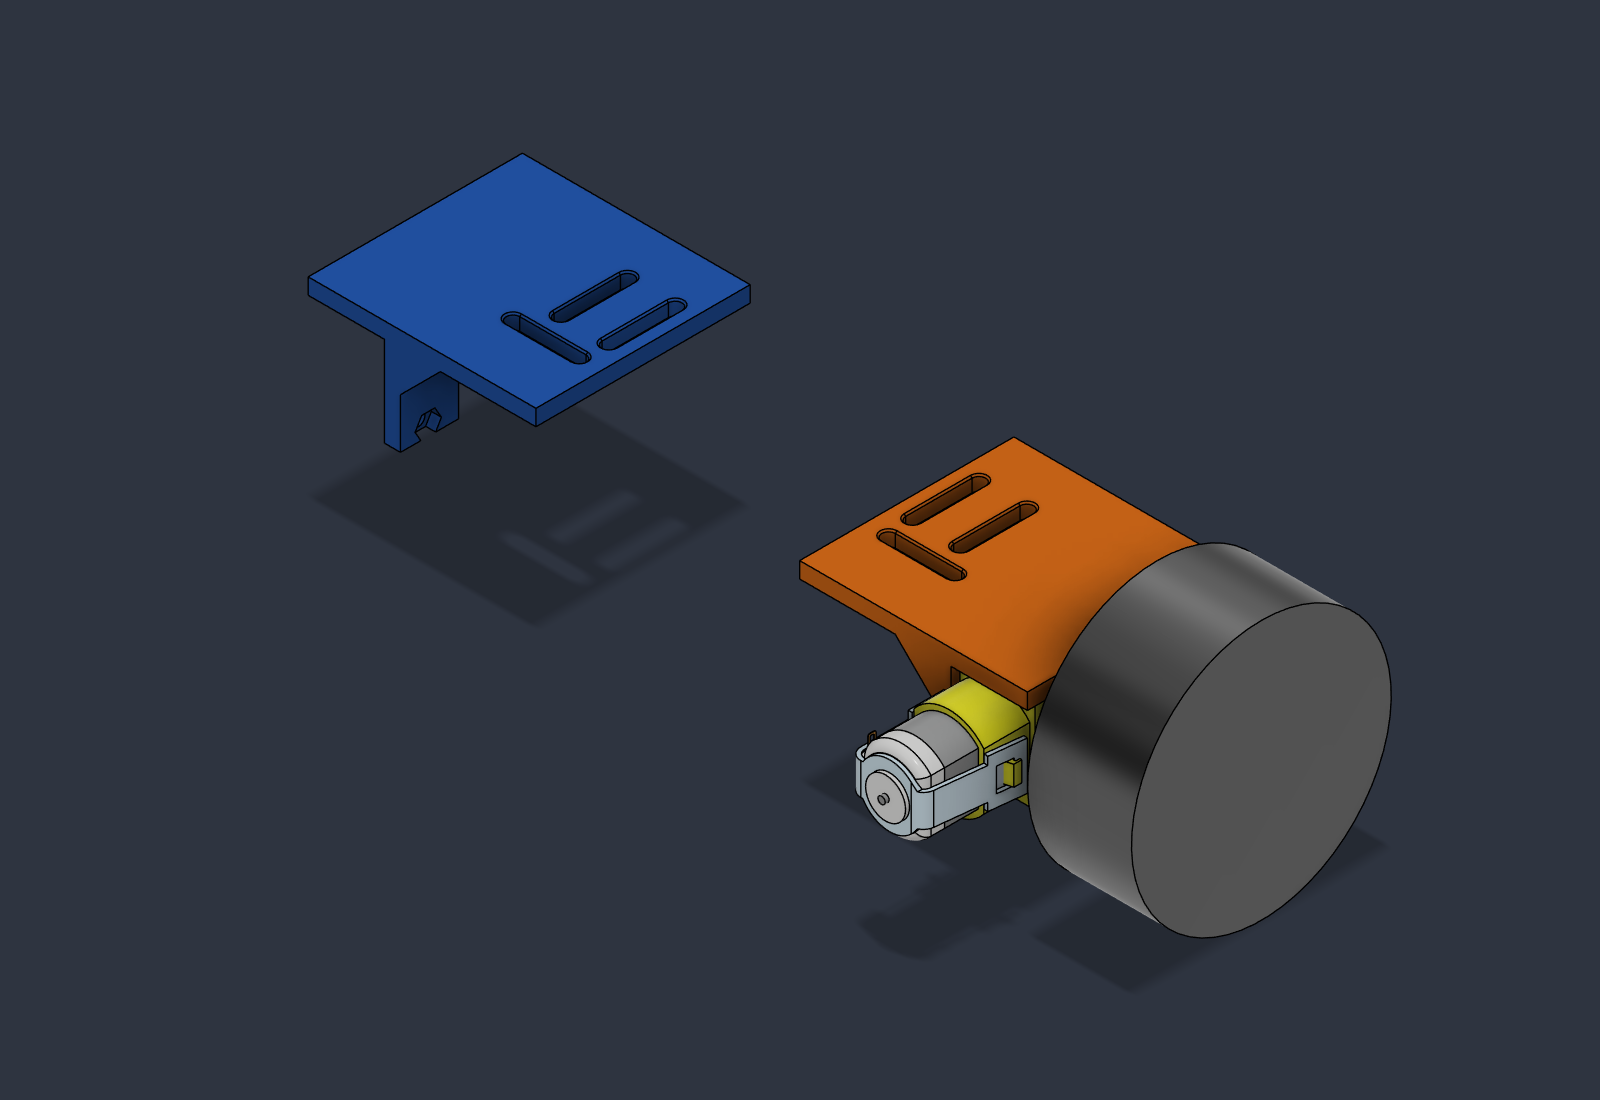
\includegraphics[width=0.85\textwidth]{shot_iso.png}
  \caption{Right and left motor brackets with the right-hand TT motor and wheel
           (isometric view).}
  \label{fig:bracket-iso}
\end{figure}

% F02 -- top view, plate hidden
\begin{figure}[htbp]
  \centering
  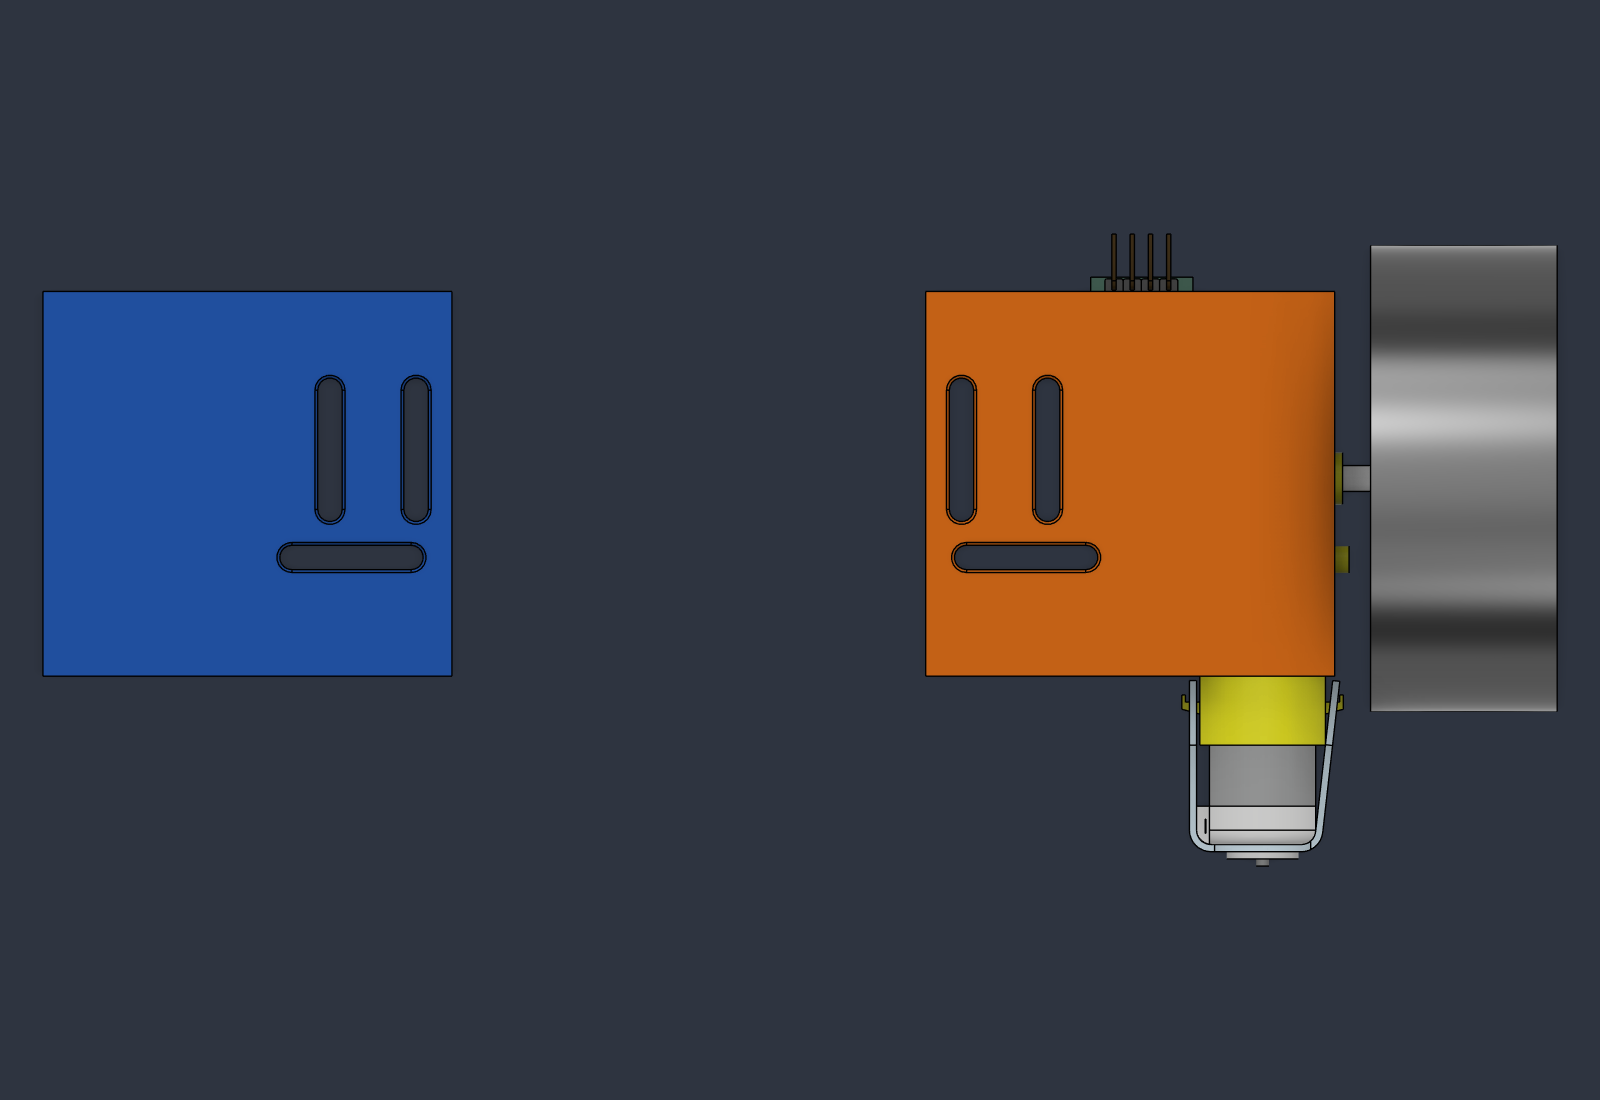
\includegraphics[width=0.85\textwidth]{shot_top.png}
  \caption{Top view of both brackets showing the three mounting slots.}
  \label{fig:bracket-top}
\end{figure}

% F03 -- Fusion "front" view (looks along +Y), plate hidden
\begin{figure}[htbp]
  \centering
  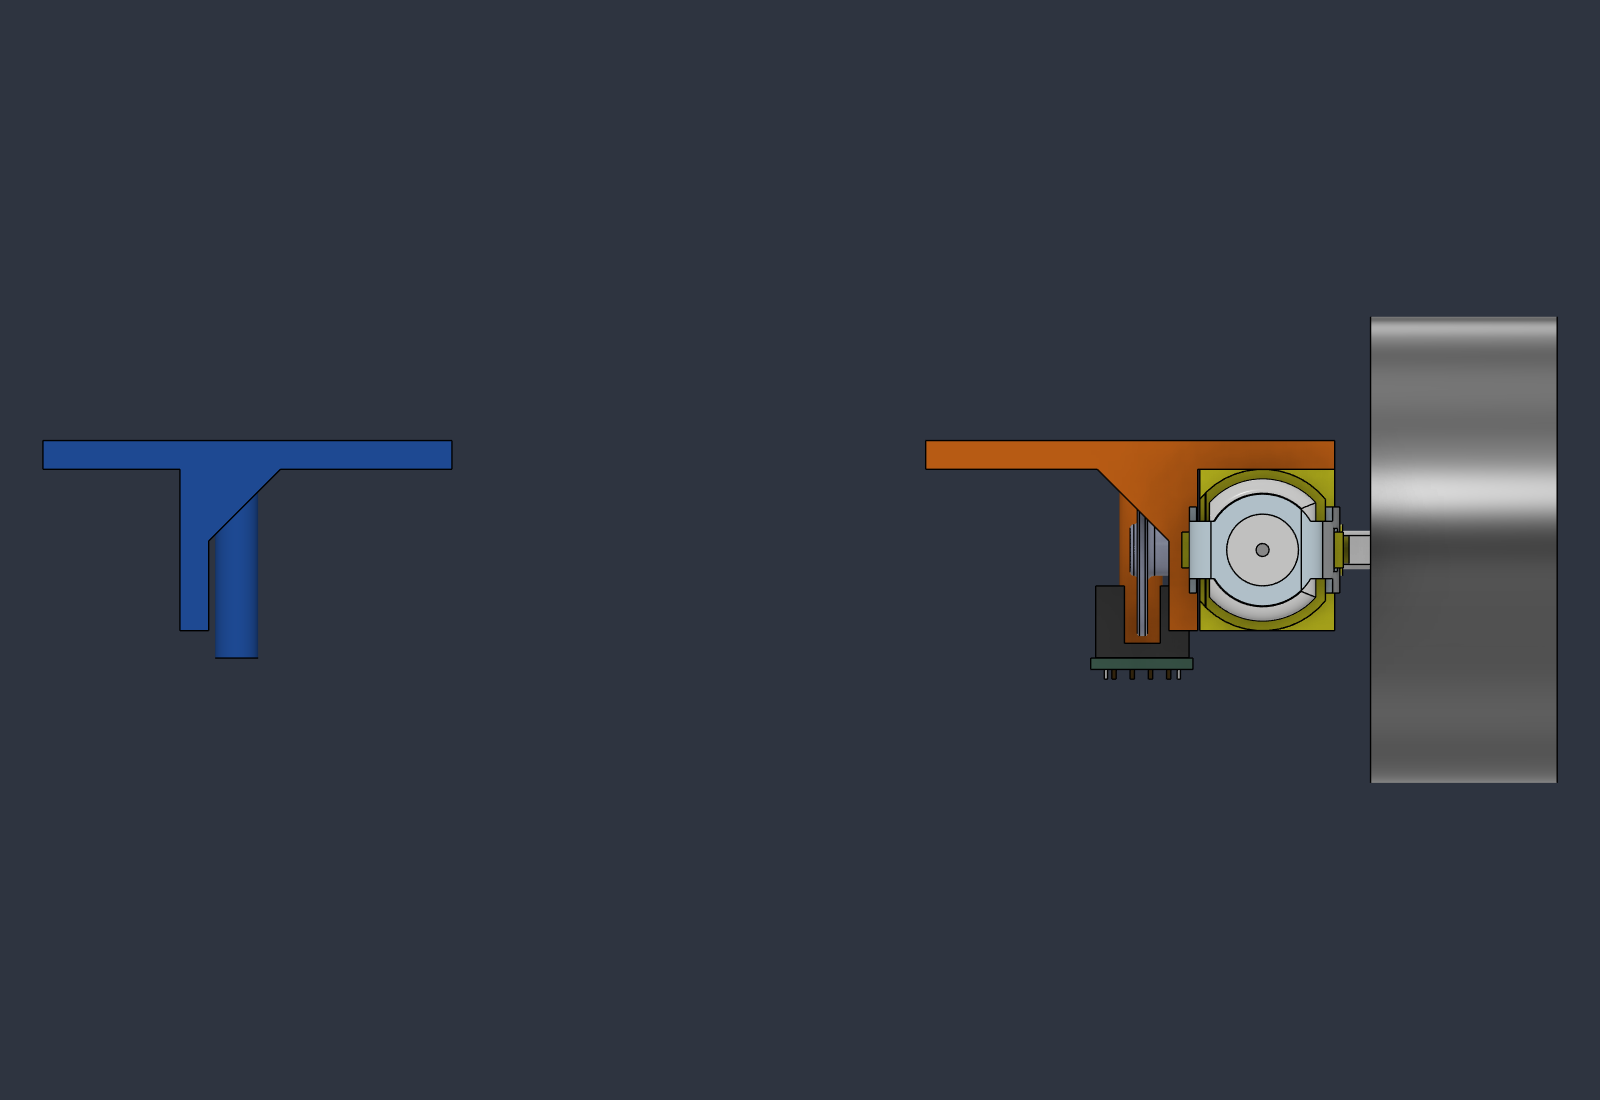
\includegraphics[width=0.85\textwidth]{shot_front.png}
  \caption{Front view: flange on the gearbox top, motor tab and sensor column.}
  \label{fig:bracket-front}
\end{figure}

% F04 -- left view, plate, wheel and left bracket hidden
\begin{figure}[htbp]
  \centering
  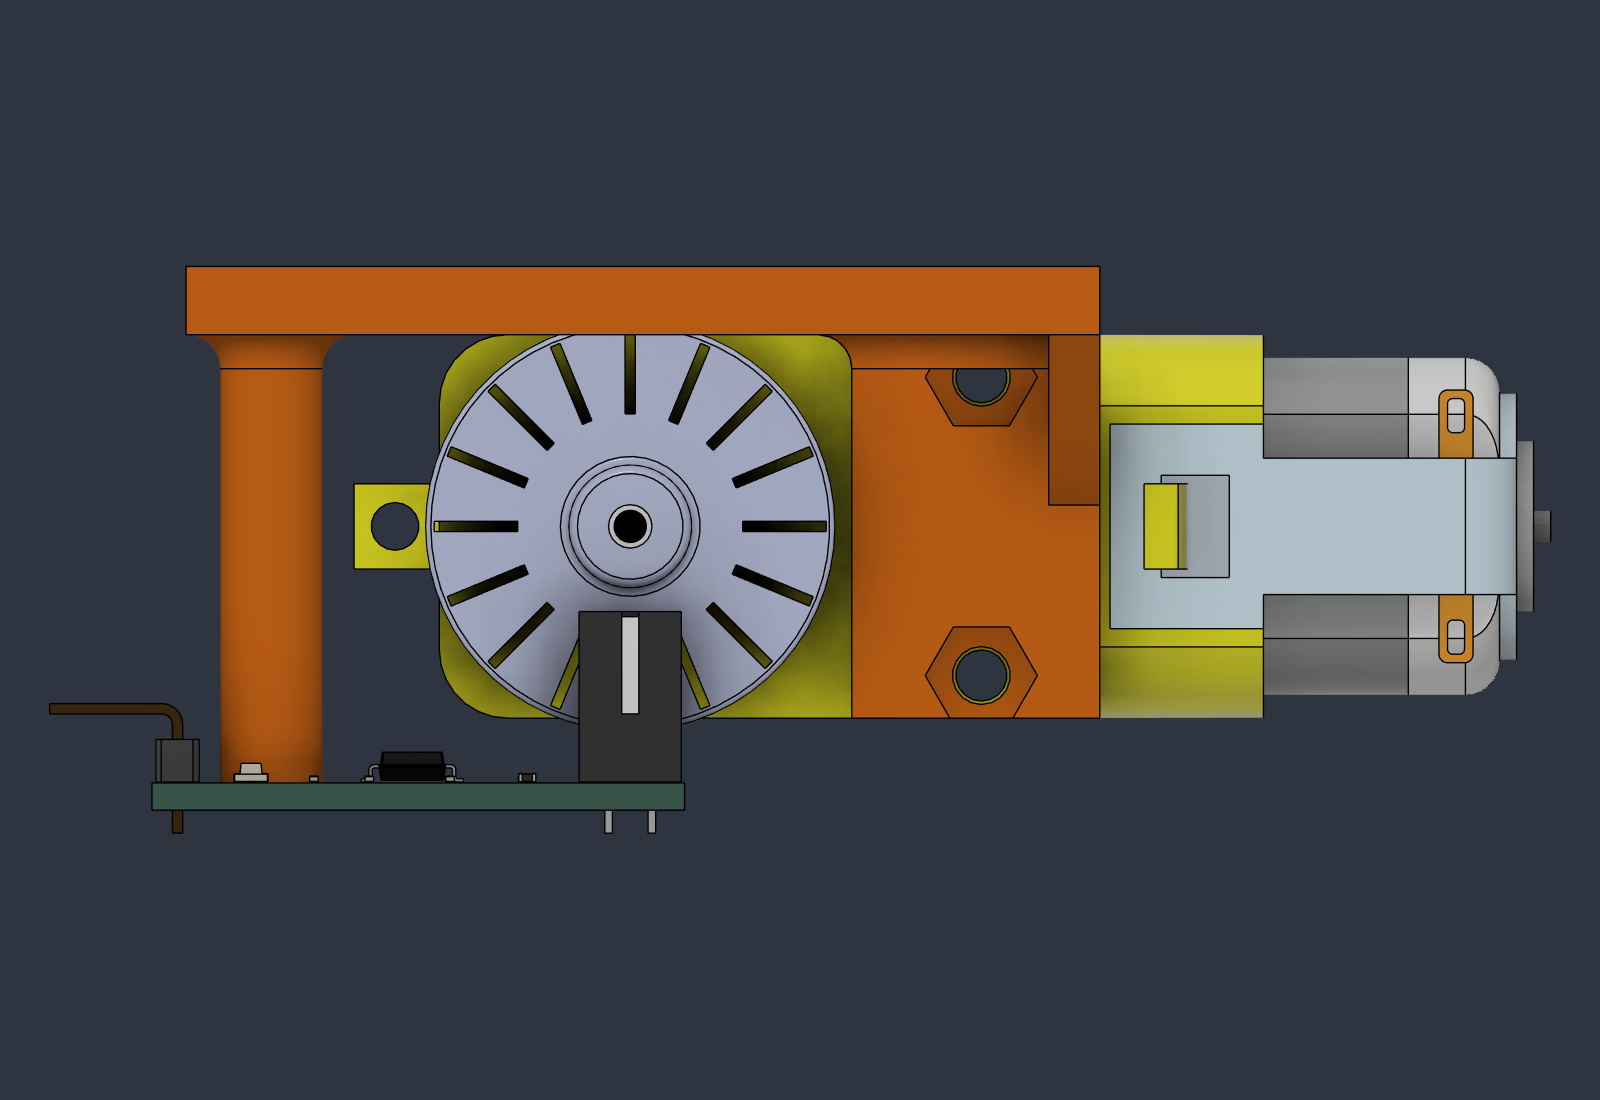
\includegraphics[width=0.85\textwidth]{shot_side.png}
  \caption{Side view: the encoder disc's bottom rim sits in the LM393 fork; the board is
           screwed to the column.}
  \label{fig:sensor-side}
\end{figure}

% F05 -- iso bottom-right view, plate shown
\begin{figure}[htbp]
  \centering
  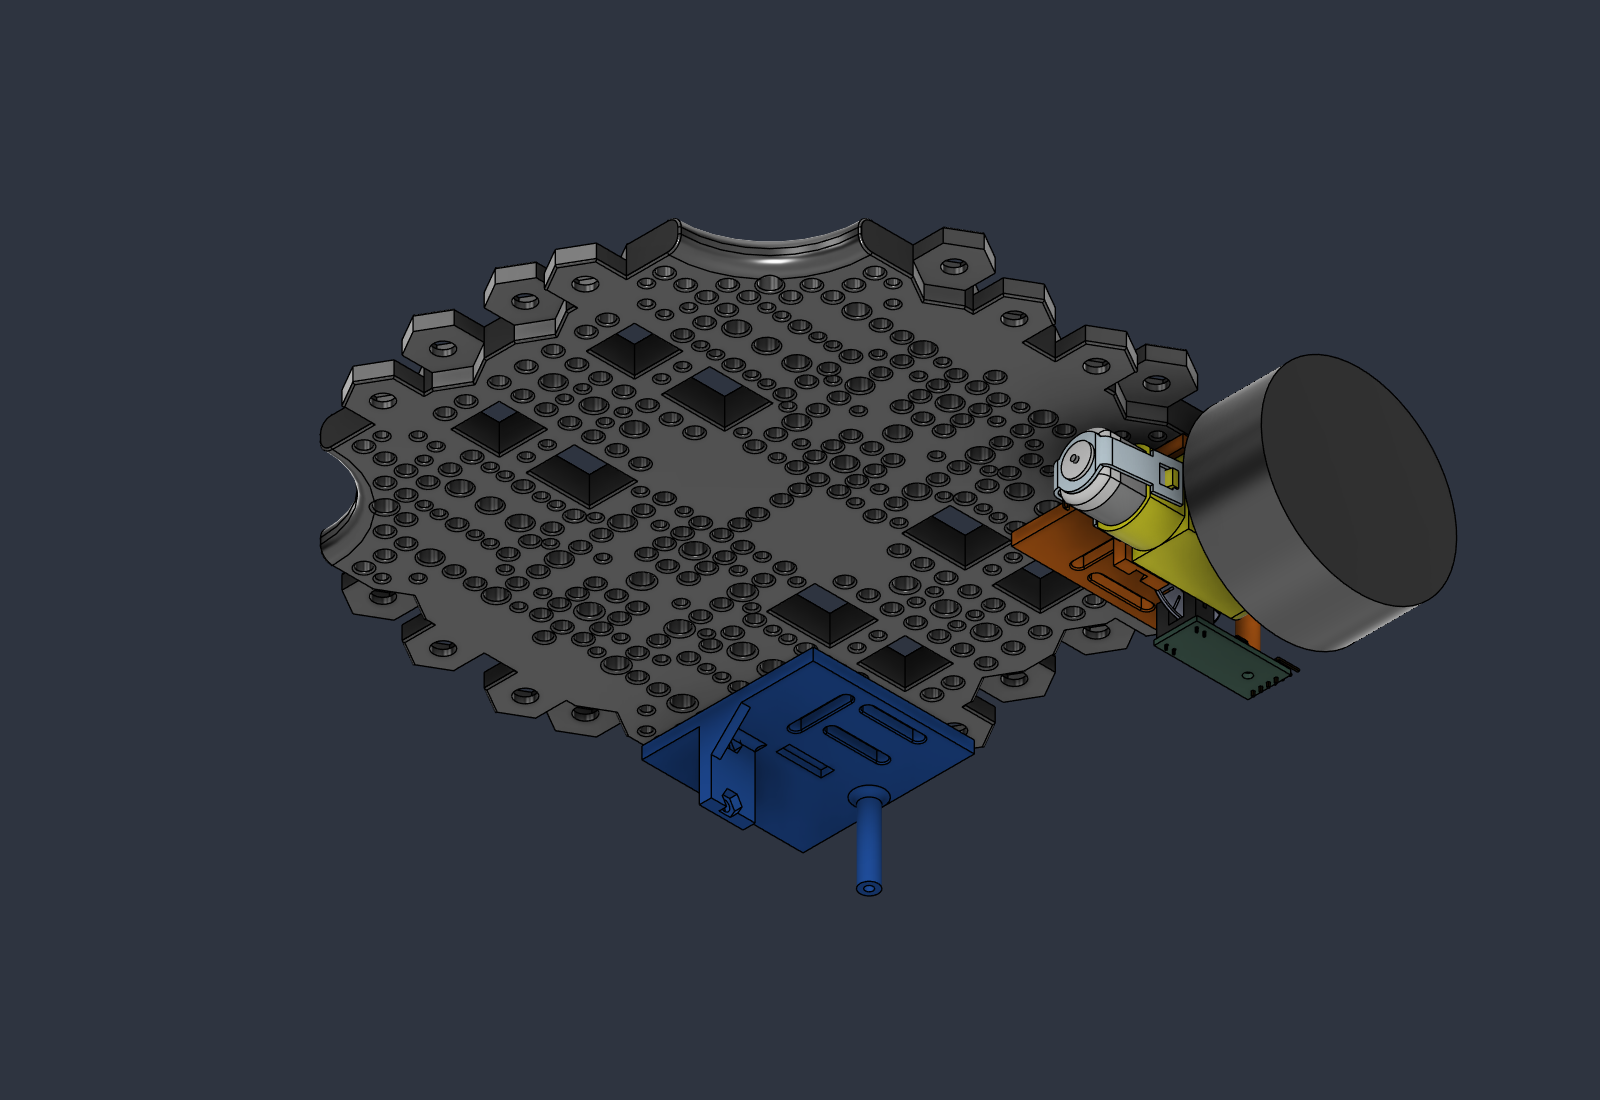
\includegraphics[width=0.85\textwidth]{shot_with_plate_below.png}
  \caption{Brackets mounted under the waffle plate, seen from below.}
  \label{fig:plate-below}
\end{figure}

% F06 -- iso top-right view, plate shown
\begin{figure}[htbp]
  \centering
  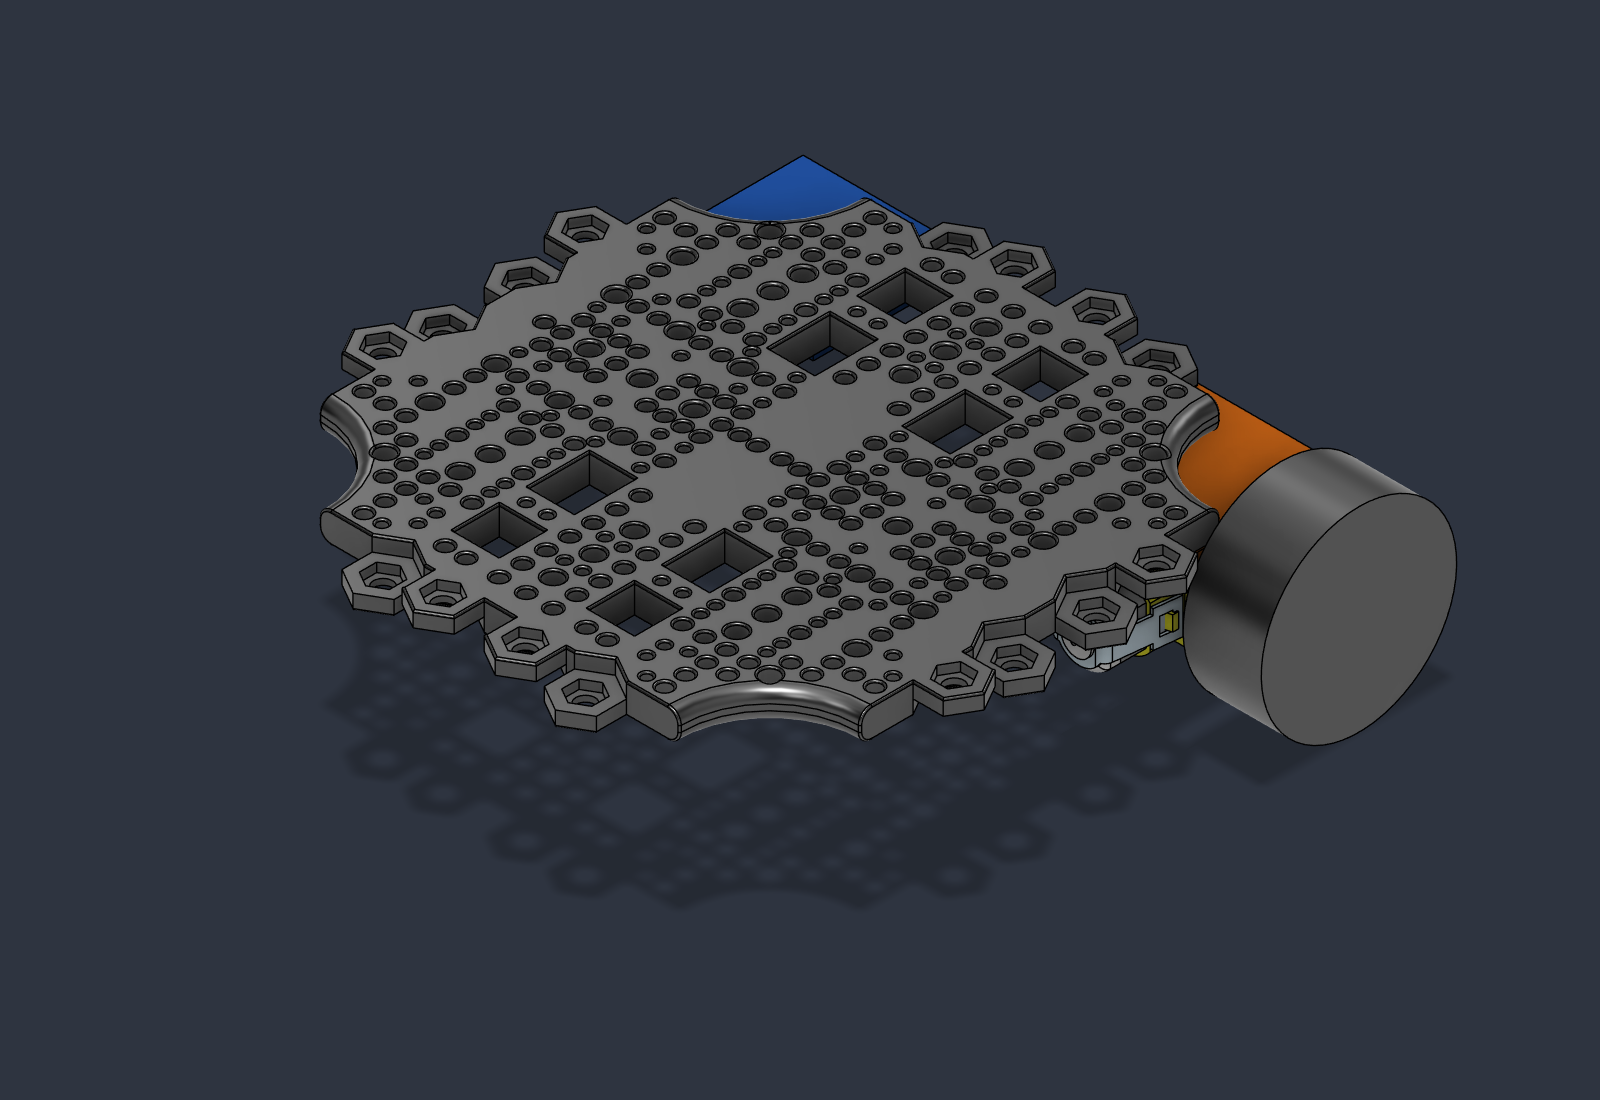
\includegraphics[width=0.85\textwidth]{shot_with_plate_top.png}
  \caption{Brackets and wheel relative to the waffle plate, seen from above.}
  \label{fig:plate-top}
\end{figure}

% F07-F10 -- bracket alone (all references hidden), four isometric views
\begin{figure}[htbp]
  \centering
  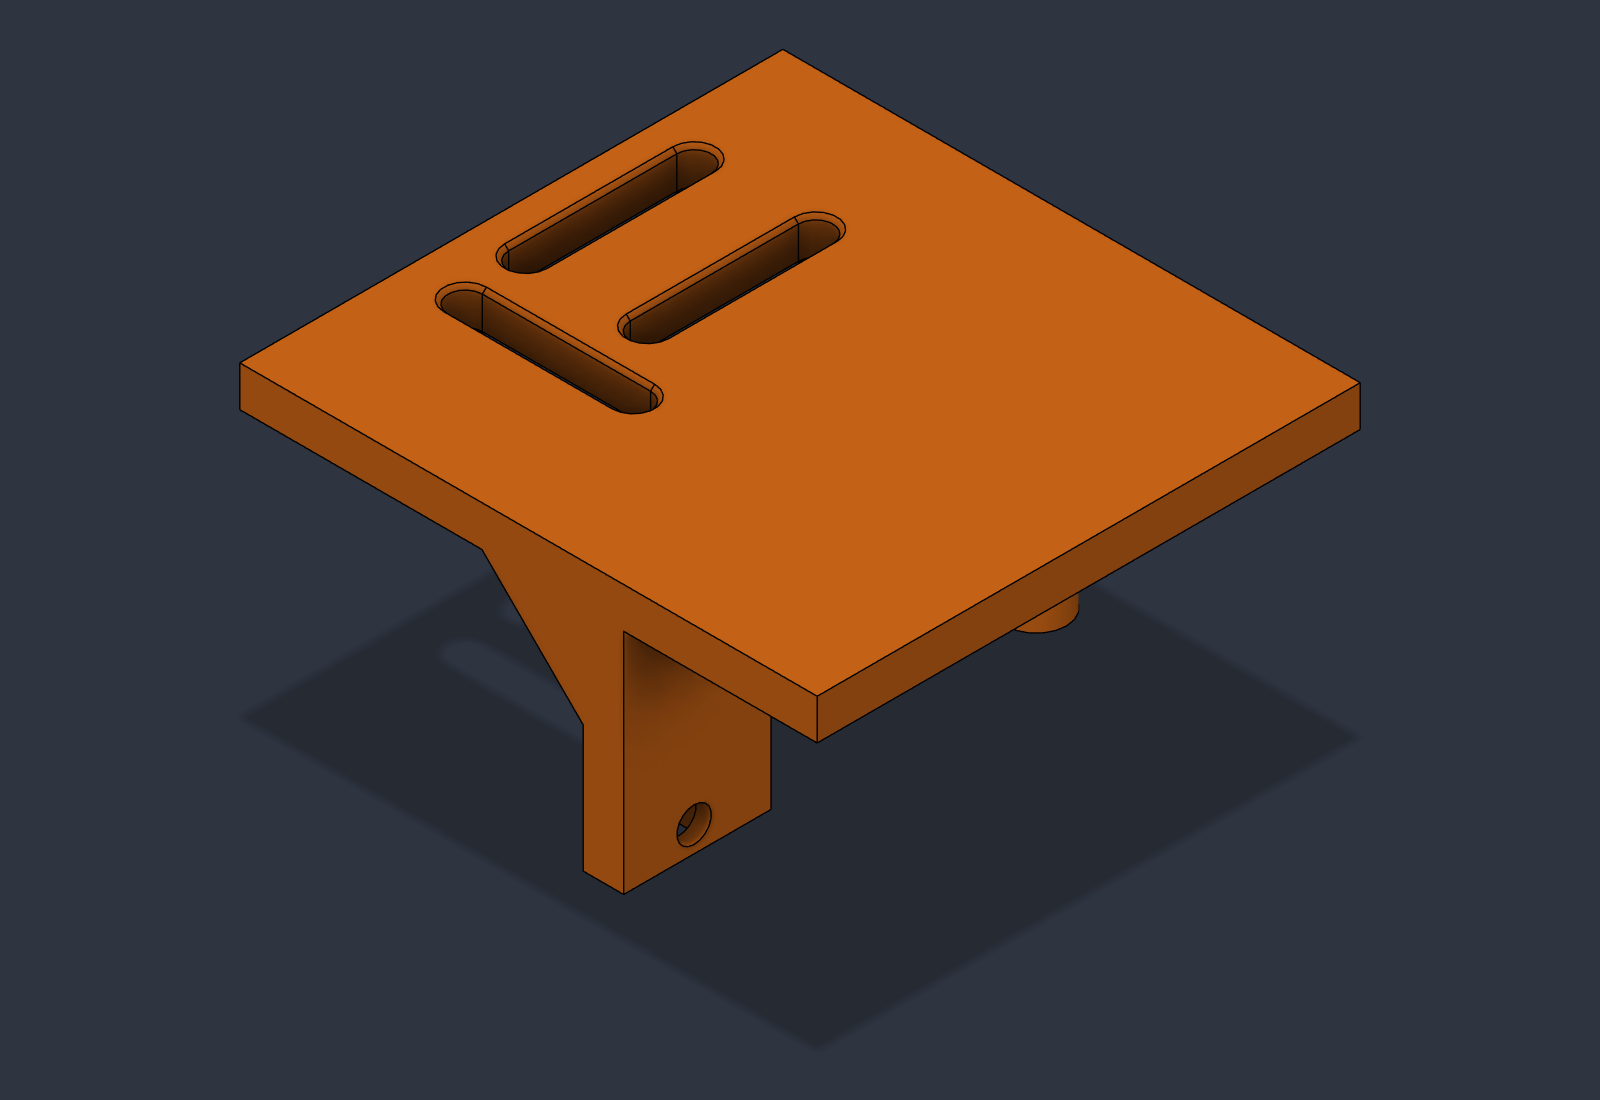
\includegraphics[width=0.48\textwidth]{angle_bracket_iso_front.png}\hfill
  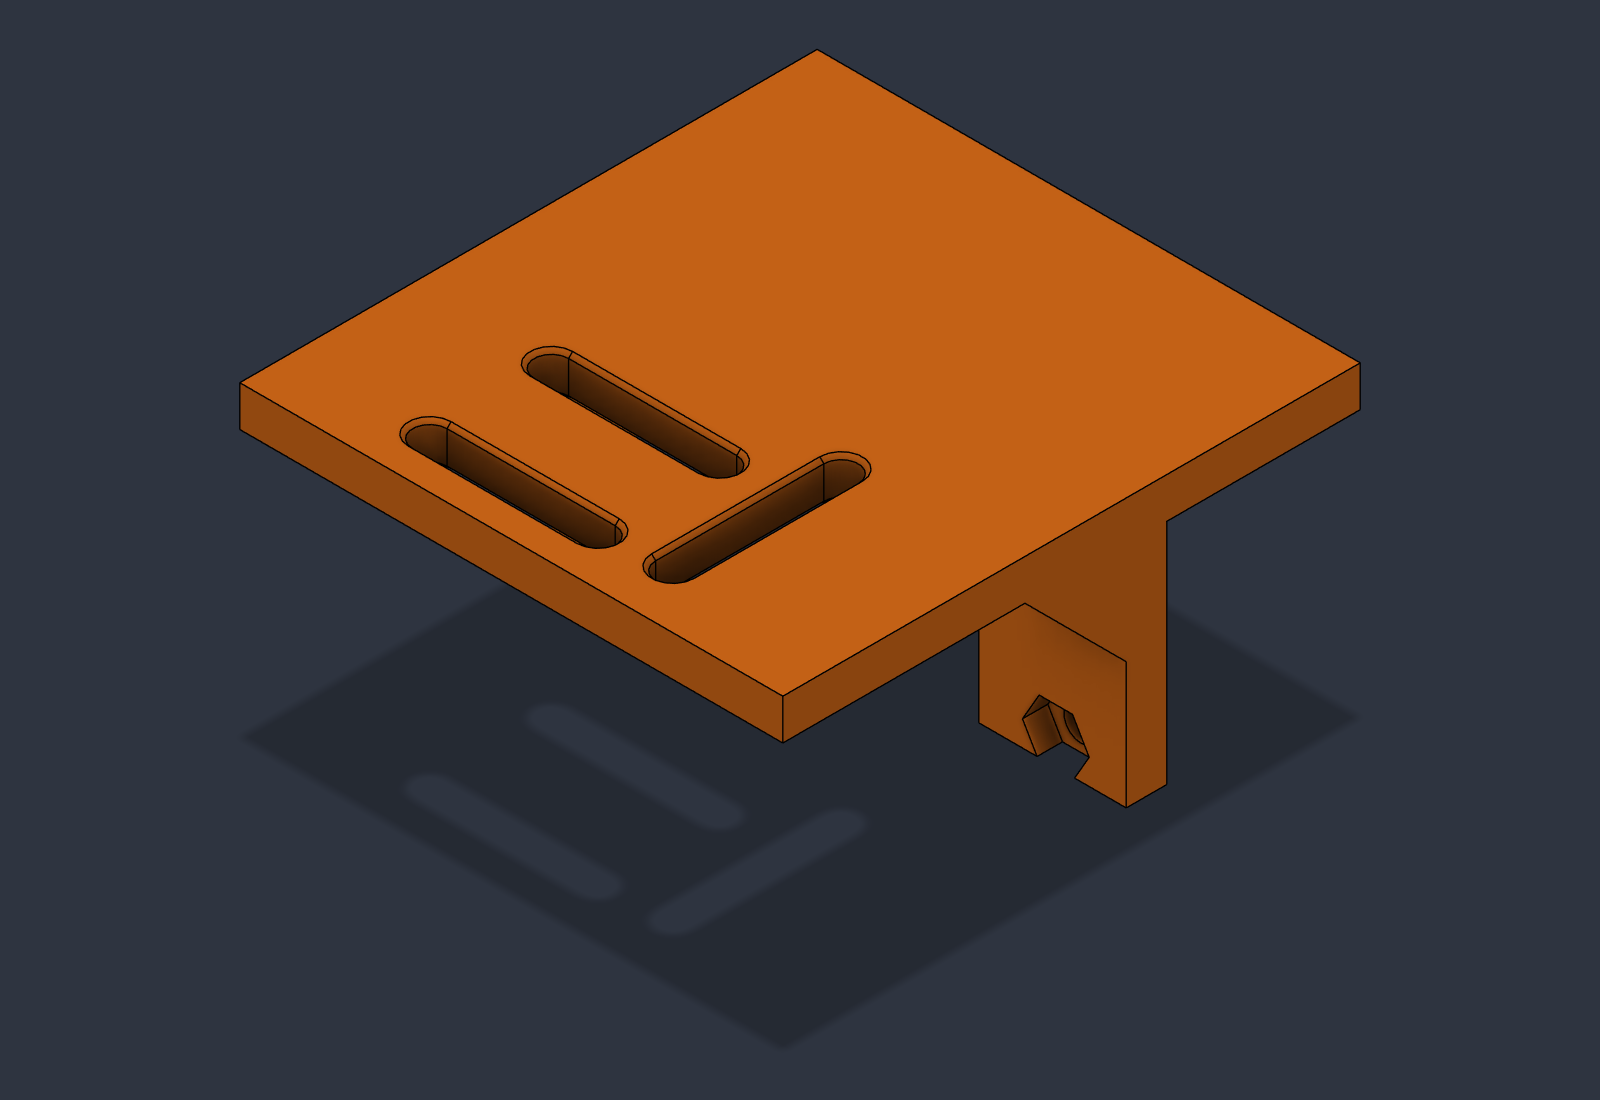
\includegraphics[width=0.48\textwidth]{angle_bracket_iso_rear.png}\\[1ex]
  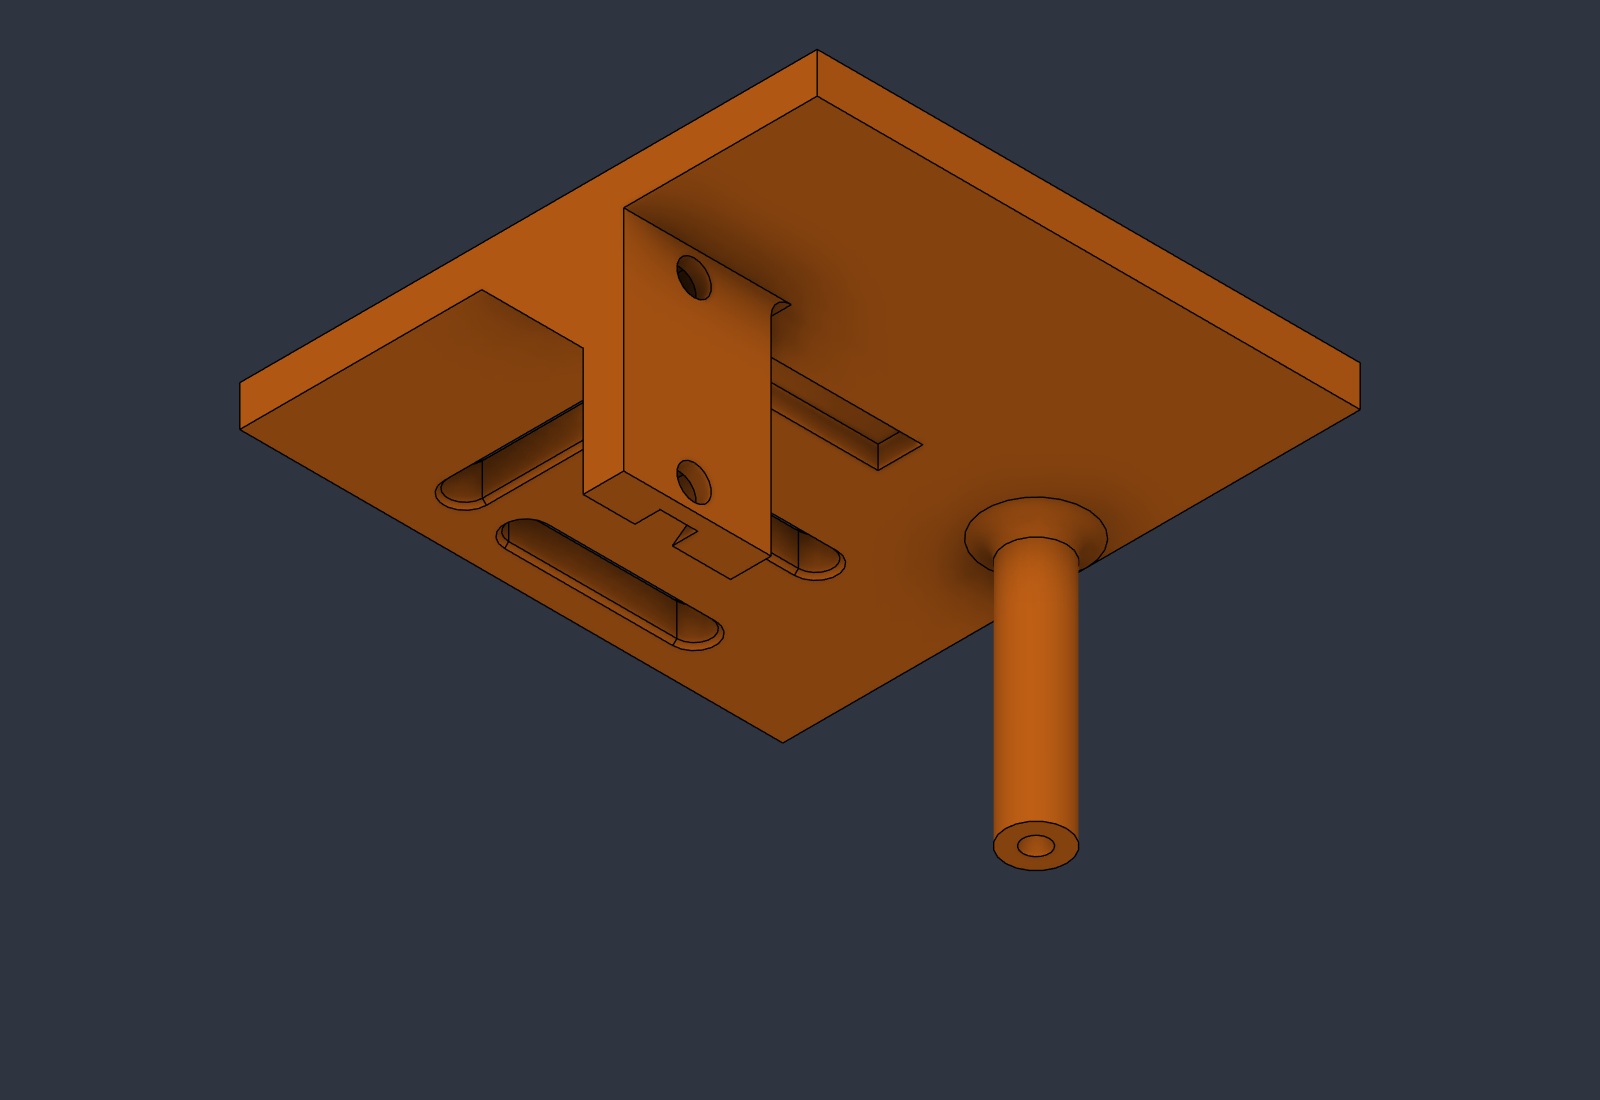
\includegraphics[width=0.48\textwidth]{angle_bracket_under_front.png}\hfill
  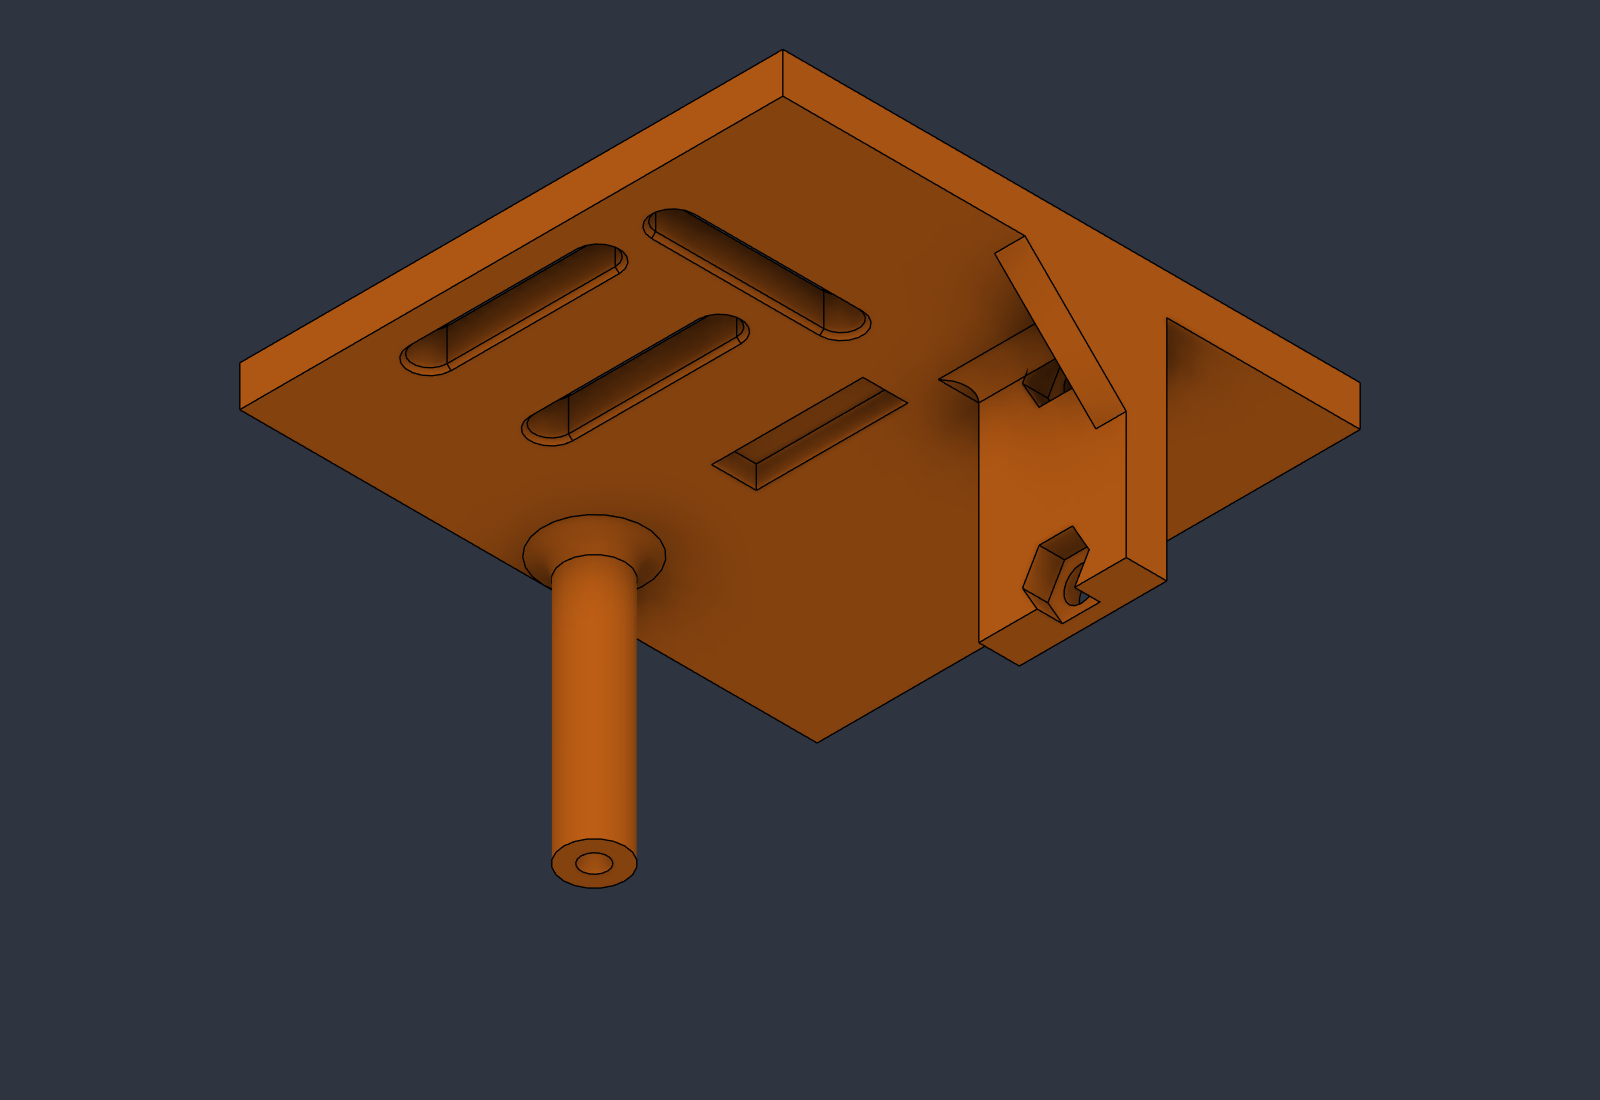
\includegraphics[width=0.48\textwidth]{angle_bracket_under_rear.png}
  \caption{Right bracket on its own: top and underside, from the front and the rear.}
  \label{fig:bracket-angles}
\end{figure}

% F11-F12 -- bracket with motor, disc and LM393 (no wheel, no plate), from below
\begin{figure}[htbp]
  \centering
  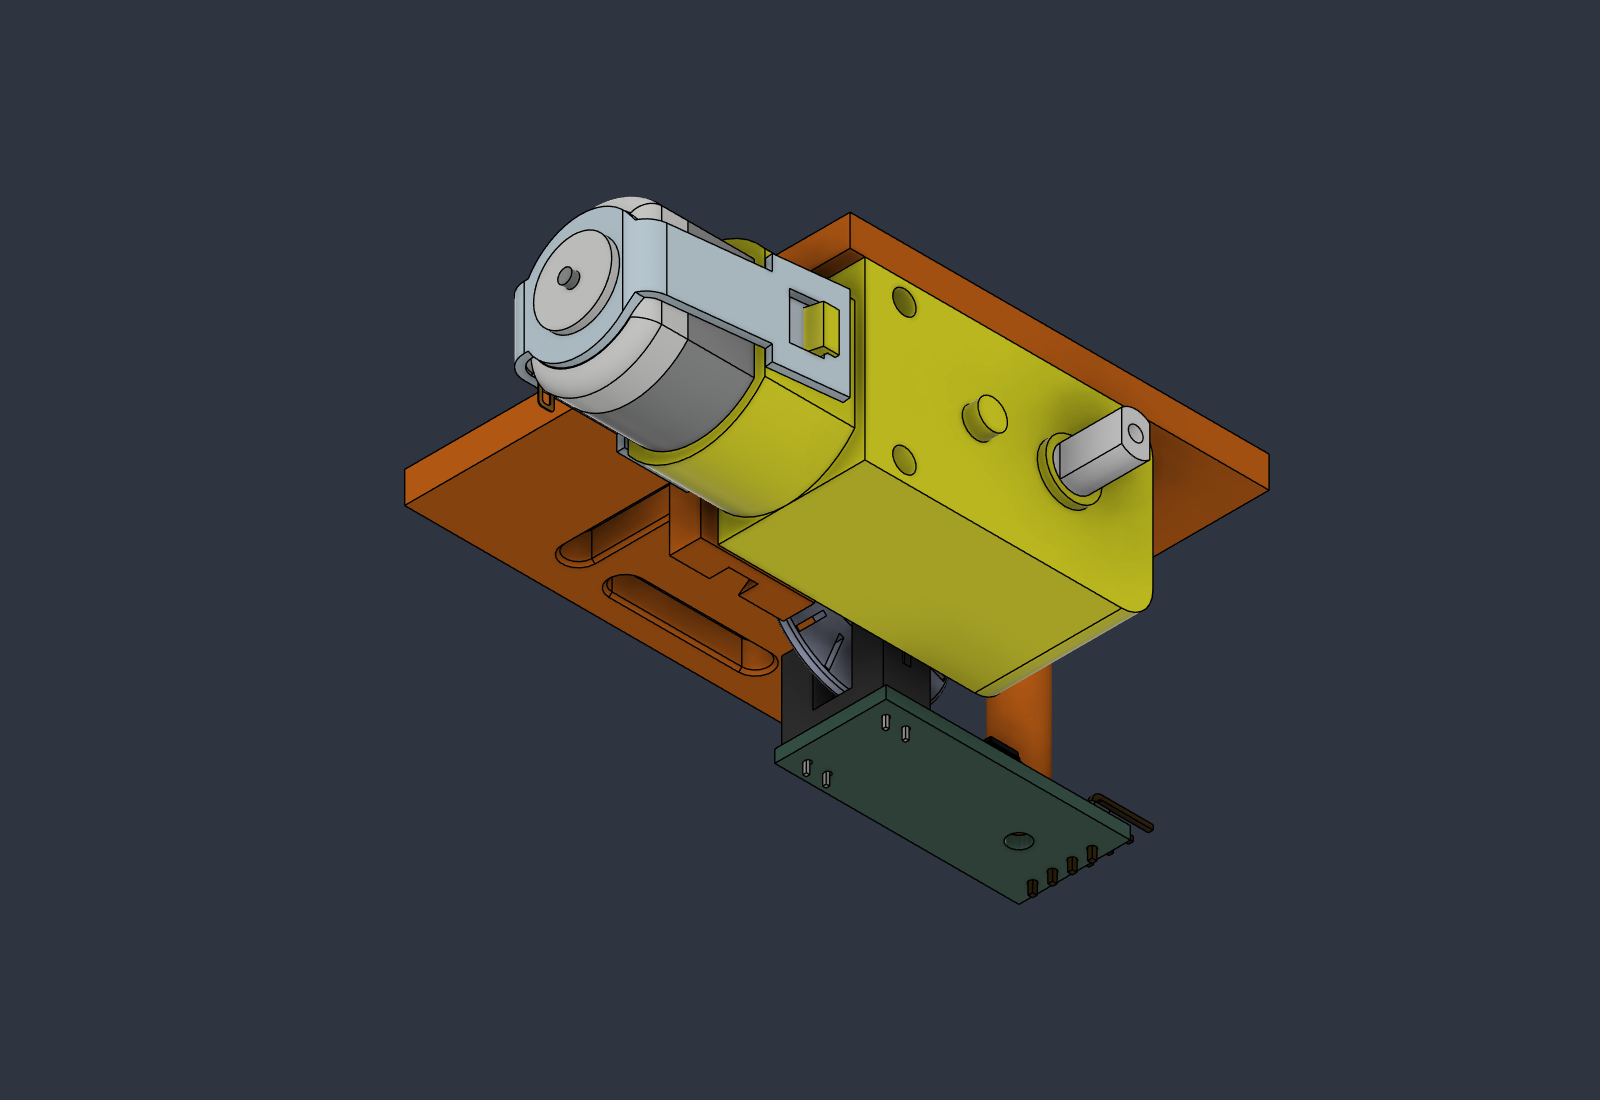
\includegraphics[width=0.48\textwidth]{angle_assembly_under_front.png}\hfill
  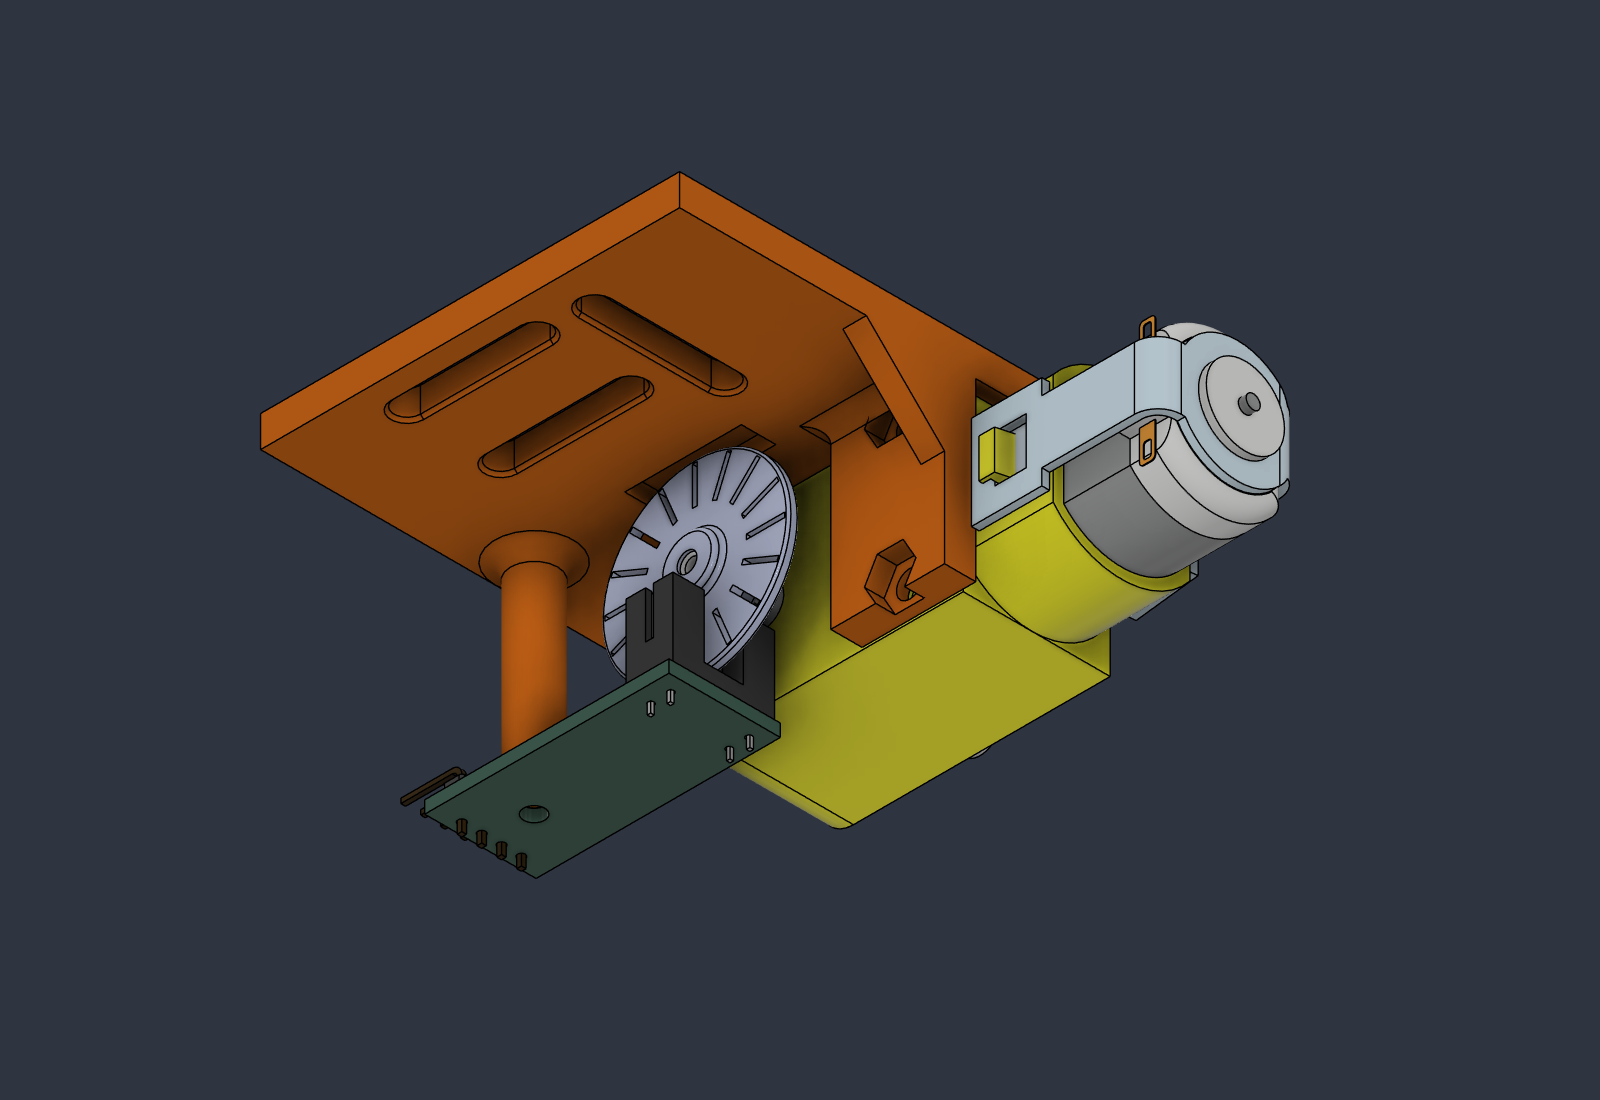
\includegraphics[width=0.48\textwidth]{angle_assembly_under_rear.png}
  \caption{Assembly from below: motor tab and nut traps, encoder disc and LM393 sensor.}
  \label{fig:assembly-below}
\end{figure}
 where needed, or copy single blocks.
% Images live in ../CAD/out/ (see \graphicspath in main.tex), so re-rendering them in
% Fusion updates the thesis without copying files.
% Every figure is also registered in tracking/log.md with how it was produced.
% Naming: label fig:<topic>-<view>.

% F01 -- made with Fusion viewport.saveAsImageFile, iso top-right view, plate hidden
\begin{figure}[htbp]
  \centering
  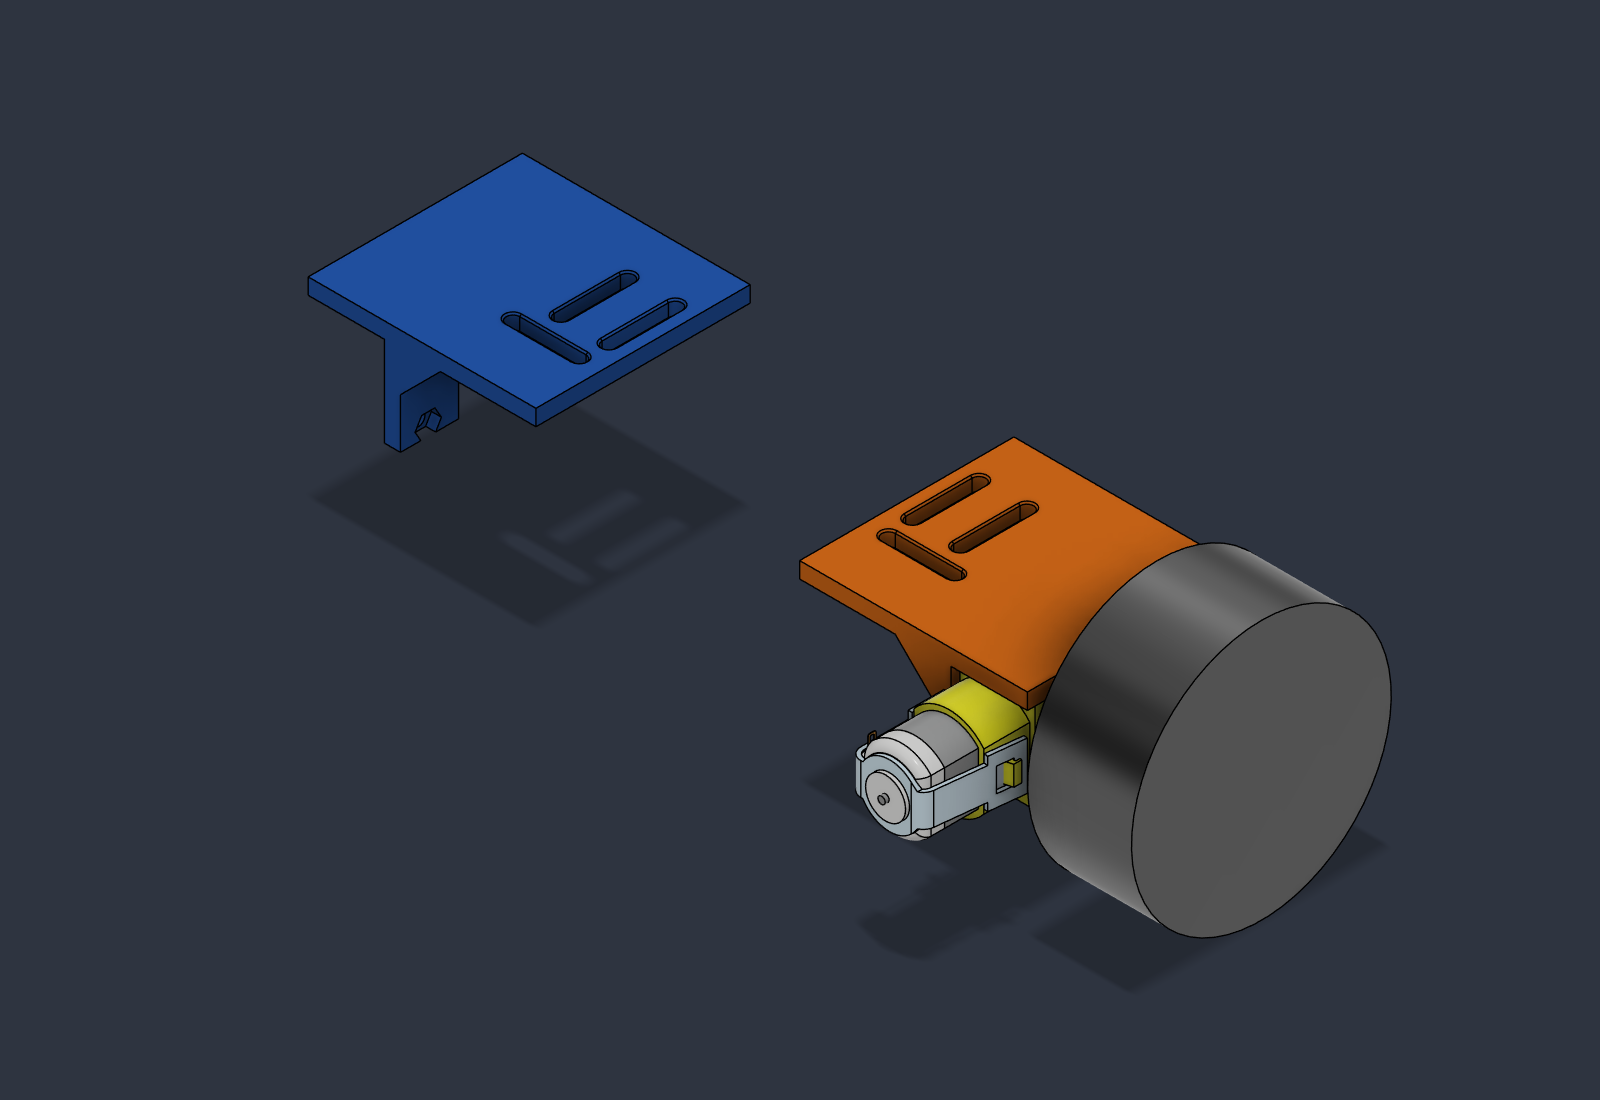
\includegraphics[width=0.85\textwidth]{shot_iso.png}
  \caption{Right and left motor brackets with the right-hand TT motor and wheel
           (isometric view).}
  \label{fig:bracket-iso}
\end{figure}

% F02 -- top view, plate hidden
\begin{figure}[htbp]
  \centering
  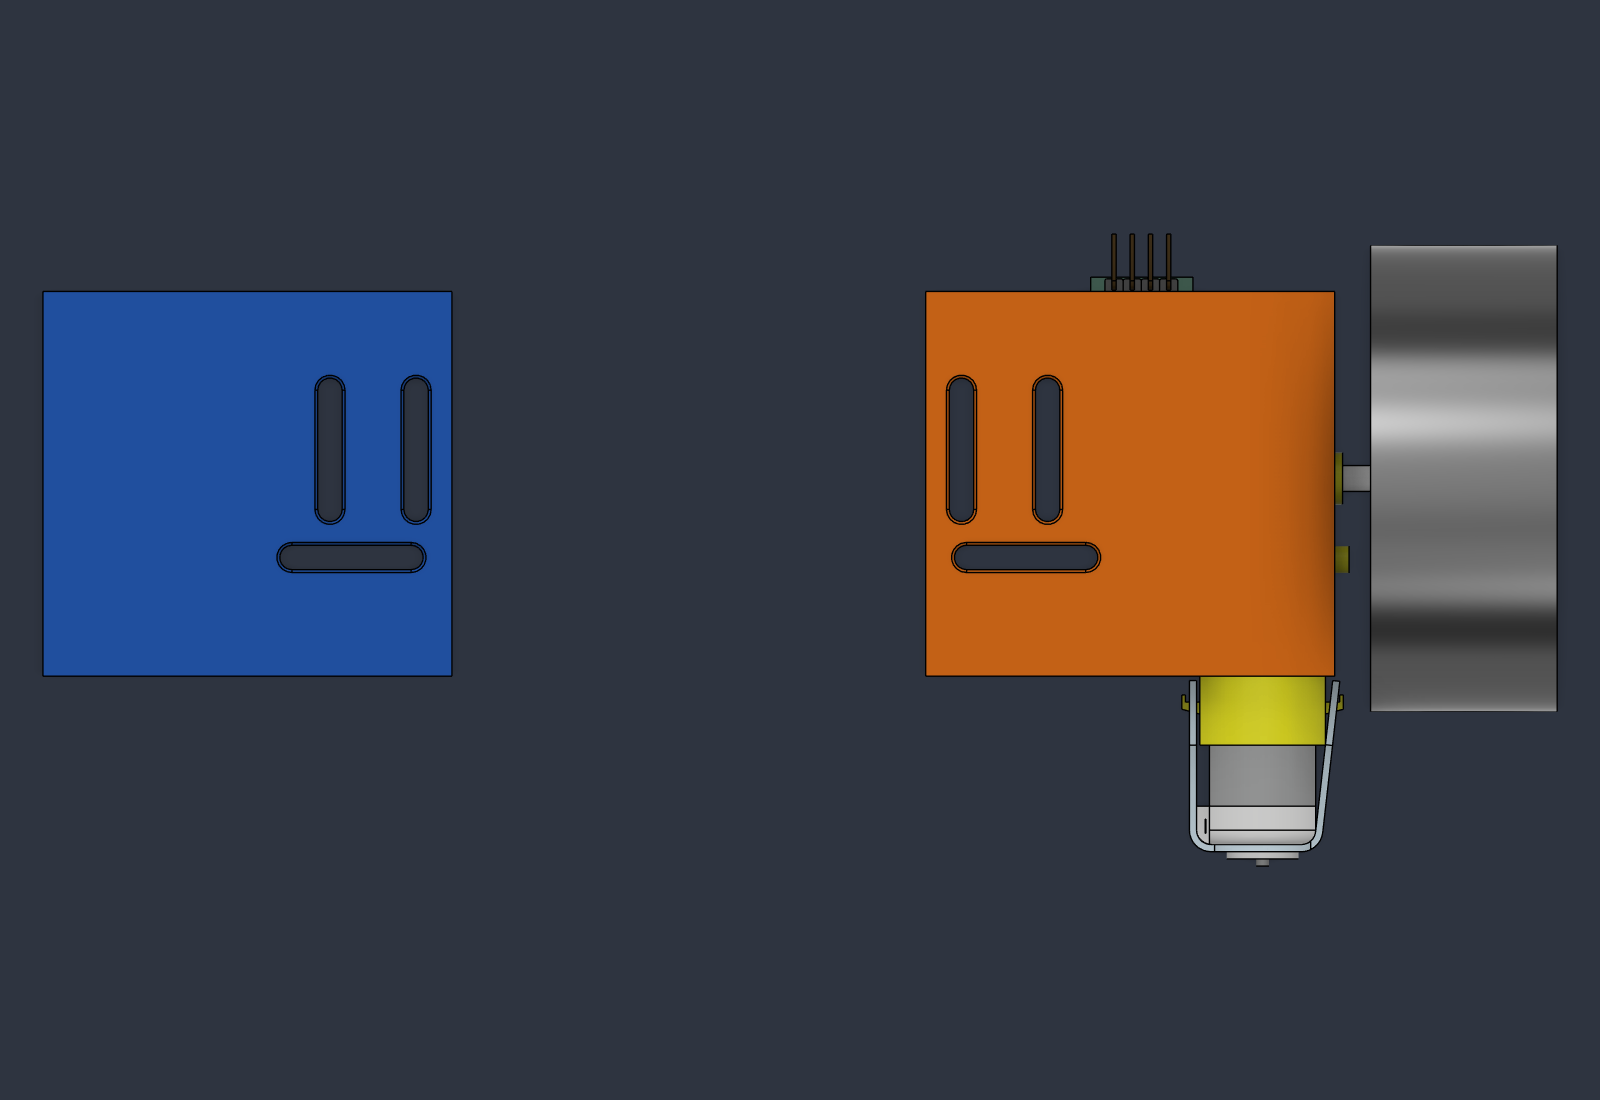
\includegraphics[width=0.85\textwidth]{shot_top.png}
  \caption{Top view of both brackets showing the three mounting slots.}
  \label{fig:bracket-top}
\end{figure}

% F03 -- Fusion "front" view (looks along +Y), plate hidden
\begin{figure}[htbp]
  \centering
  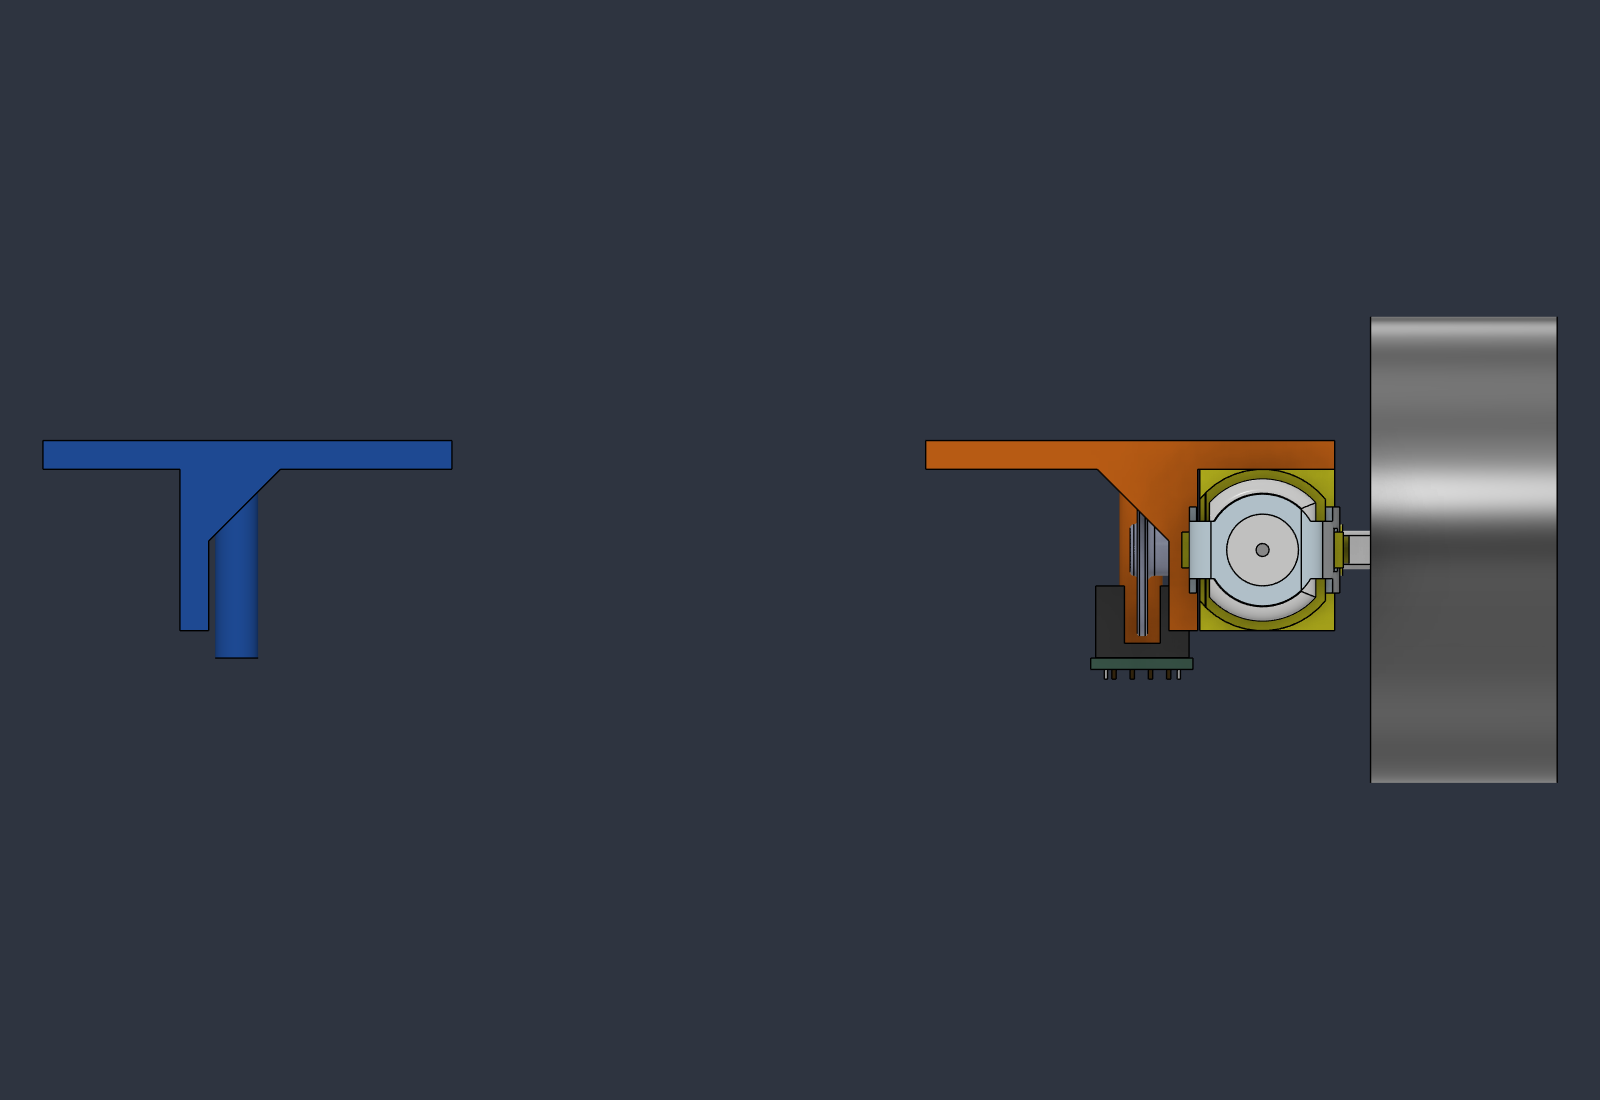
\includegraphics[width=0.85\textwidth]{shot_front.png}
  \caption{Front view: flange on the gearbox top, motor tab and sensor column.}
  \label{fig:bracket-front}
\end{figure}

% F04 -- left view, plate, wheel and left bracket hidden
\begin{figure}[htbp]
  \centering
  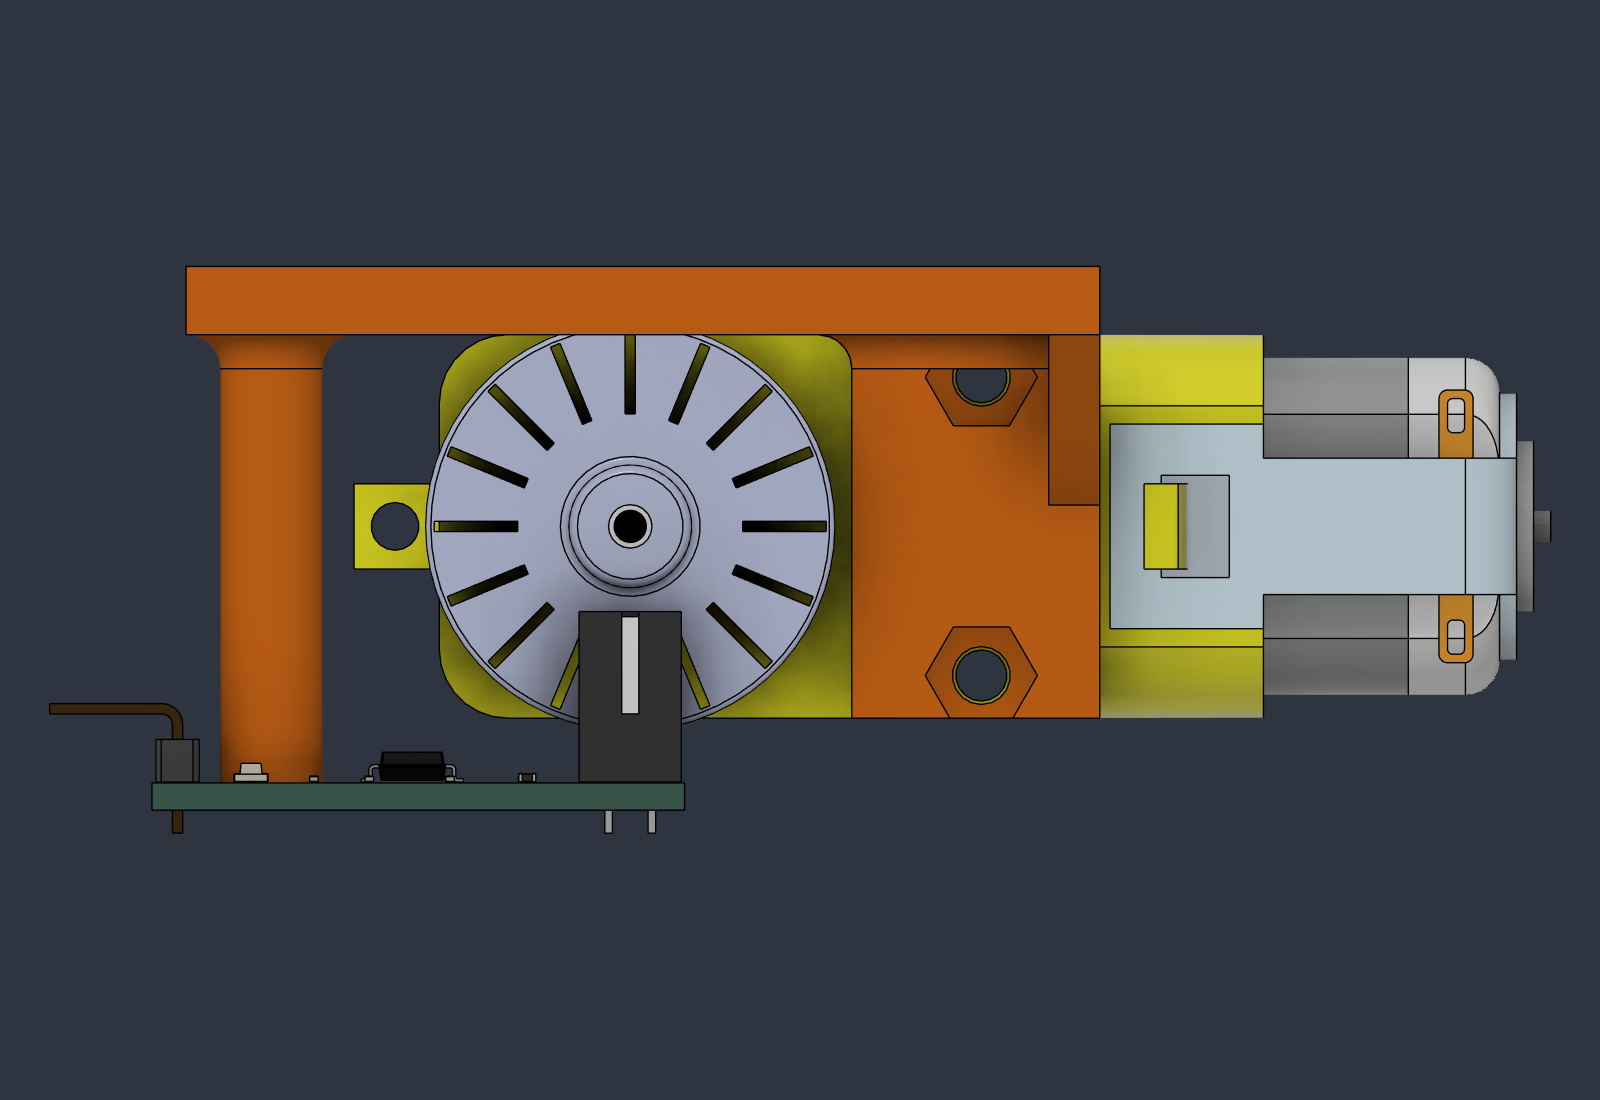
\includegraphics[width=0.85\textwidth]{shot_side.png}
  \caption{Side view: the encoder disc's bottom rim sits in the LM393 fork; the board is
           screwed to the column.}
  \label{fig:sensor-side}
\end{figure}

% F05 -- iso bottom-right view, plate shown
\begin{figure}[htbp]
  \centering
  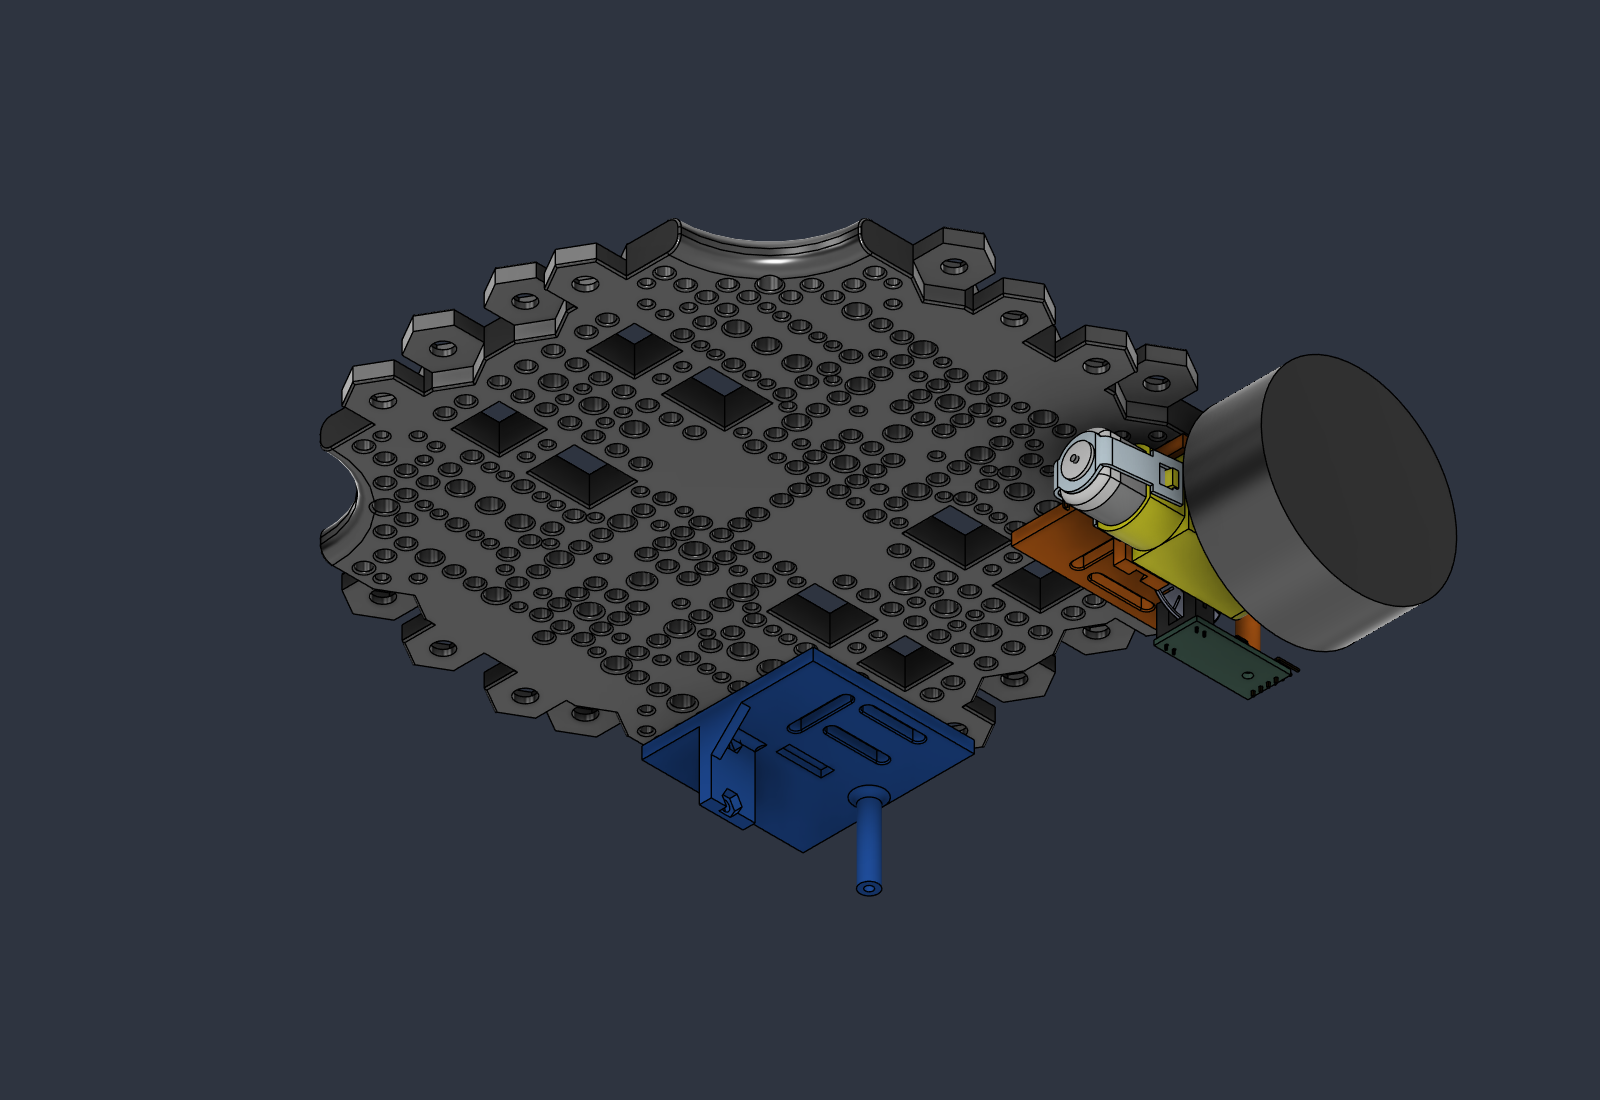
\includegraphics[width=0.85\textwidth]{shot_with_plate_below.png}
  \caption{Brackets mounted under the waffle plate, seen from below.}
  \label{fig:plate-below}
\end{figure}

% F06 -- iso top-right view, plate shown
\begin{figure}[htbp]
  \centering
  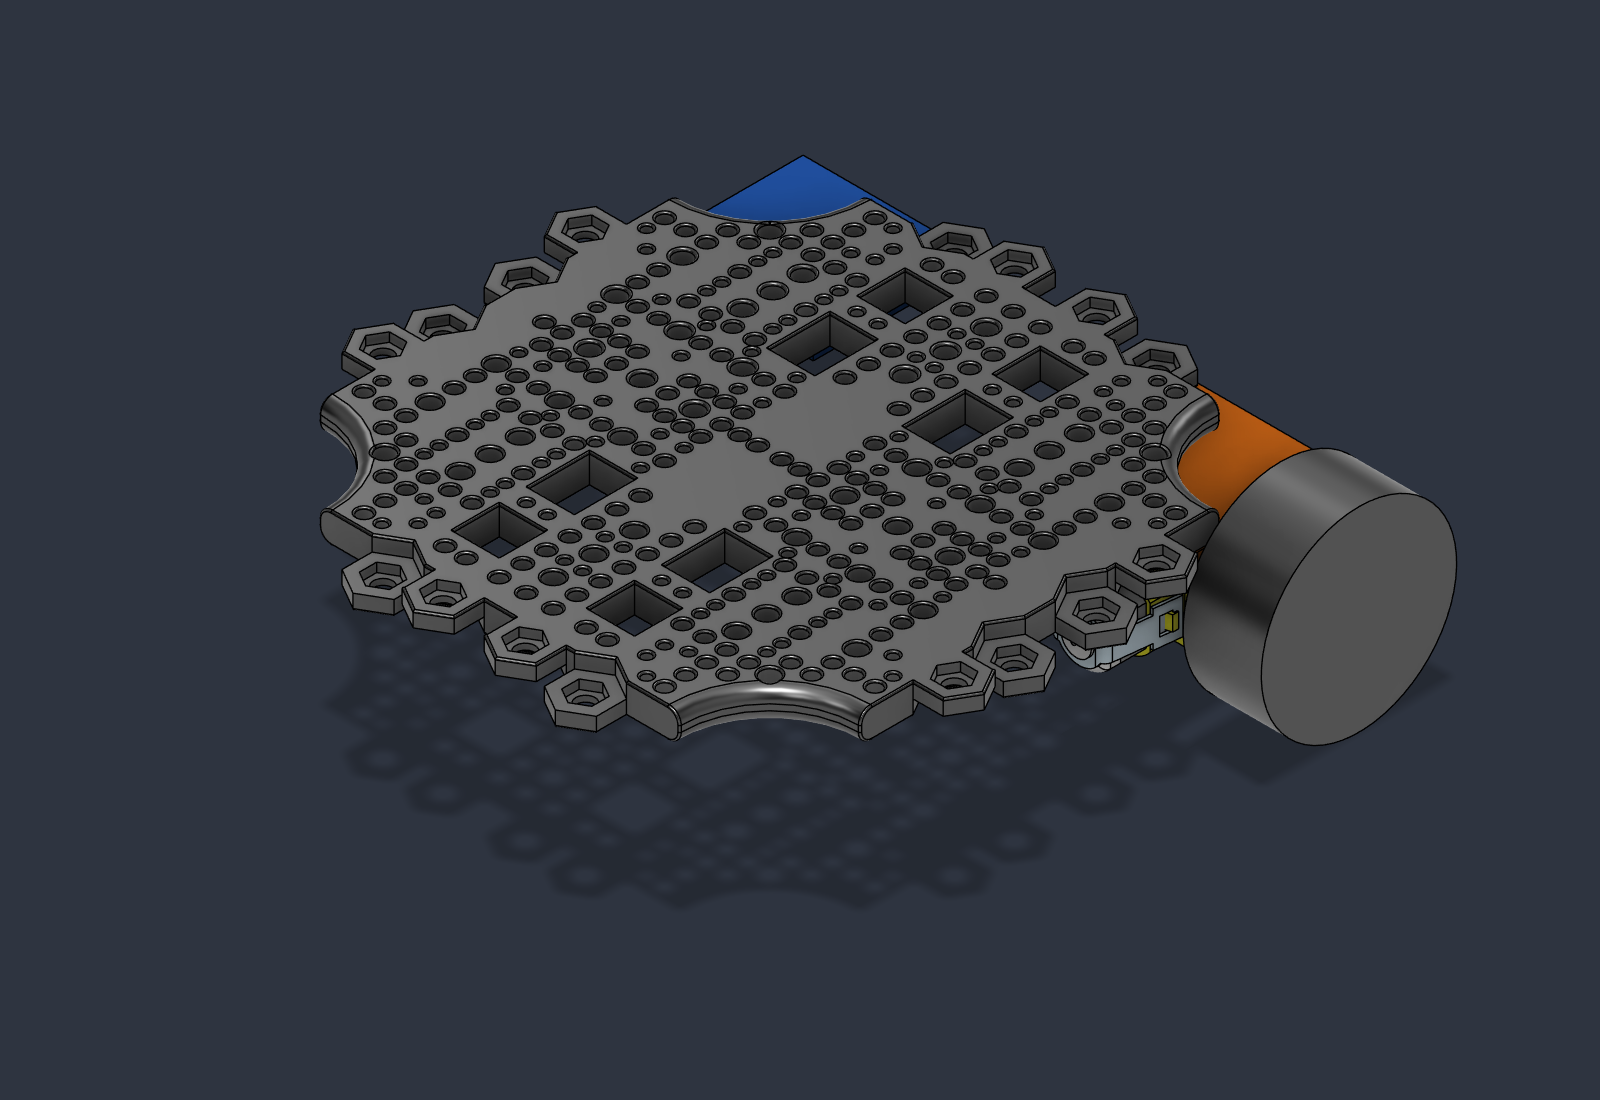
\includegraphics[width=0.85\textwidth]{shot_with_plate_top.png}
  \caption{Brackets and wheel relative to the waffle plate, seen from above.}
  \label{fig:plate-top}
\end{figure}

% F07-F10 -- bracket alone (all references hidden), four isometric views
\begin{figure}[htbp]
  \centering
  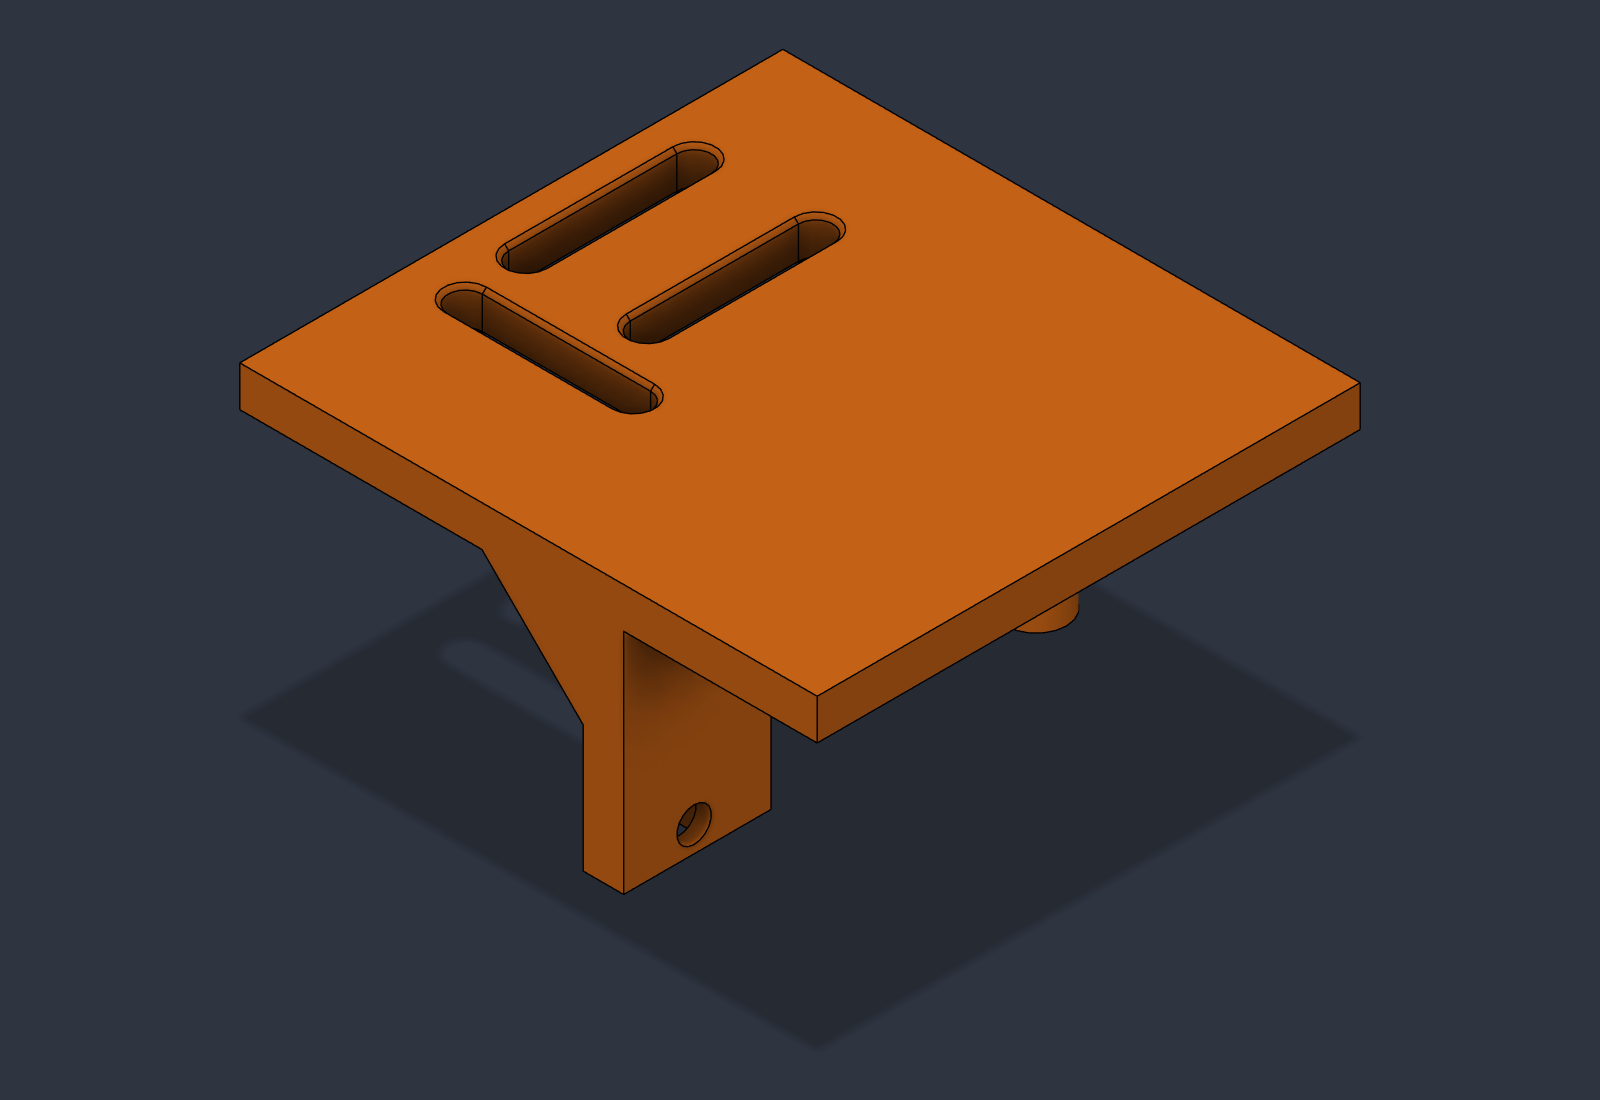
\includegraphics[width=0.48\textwidth]{angle_bracket_iso_front.png}\hfill
  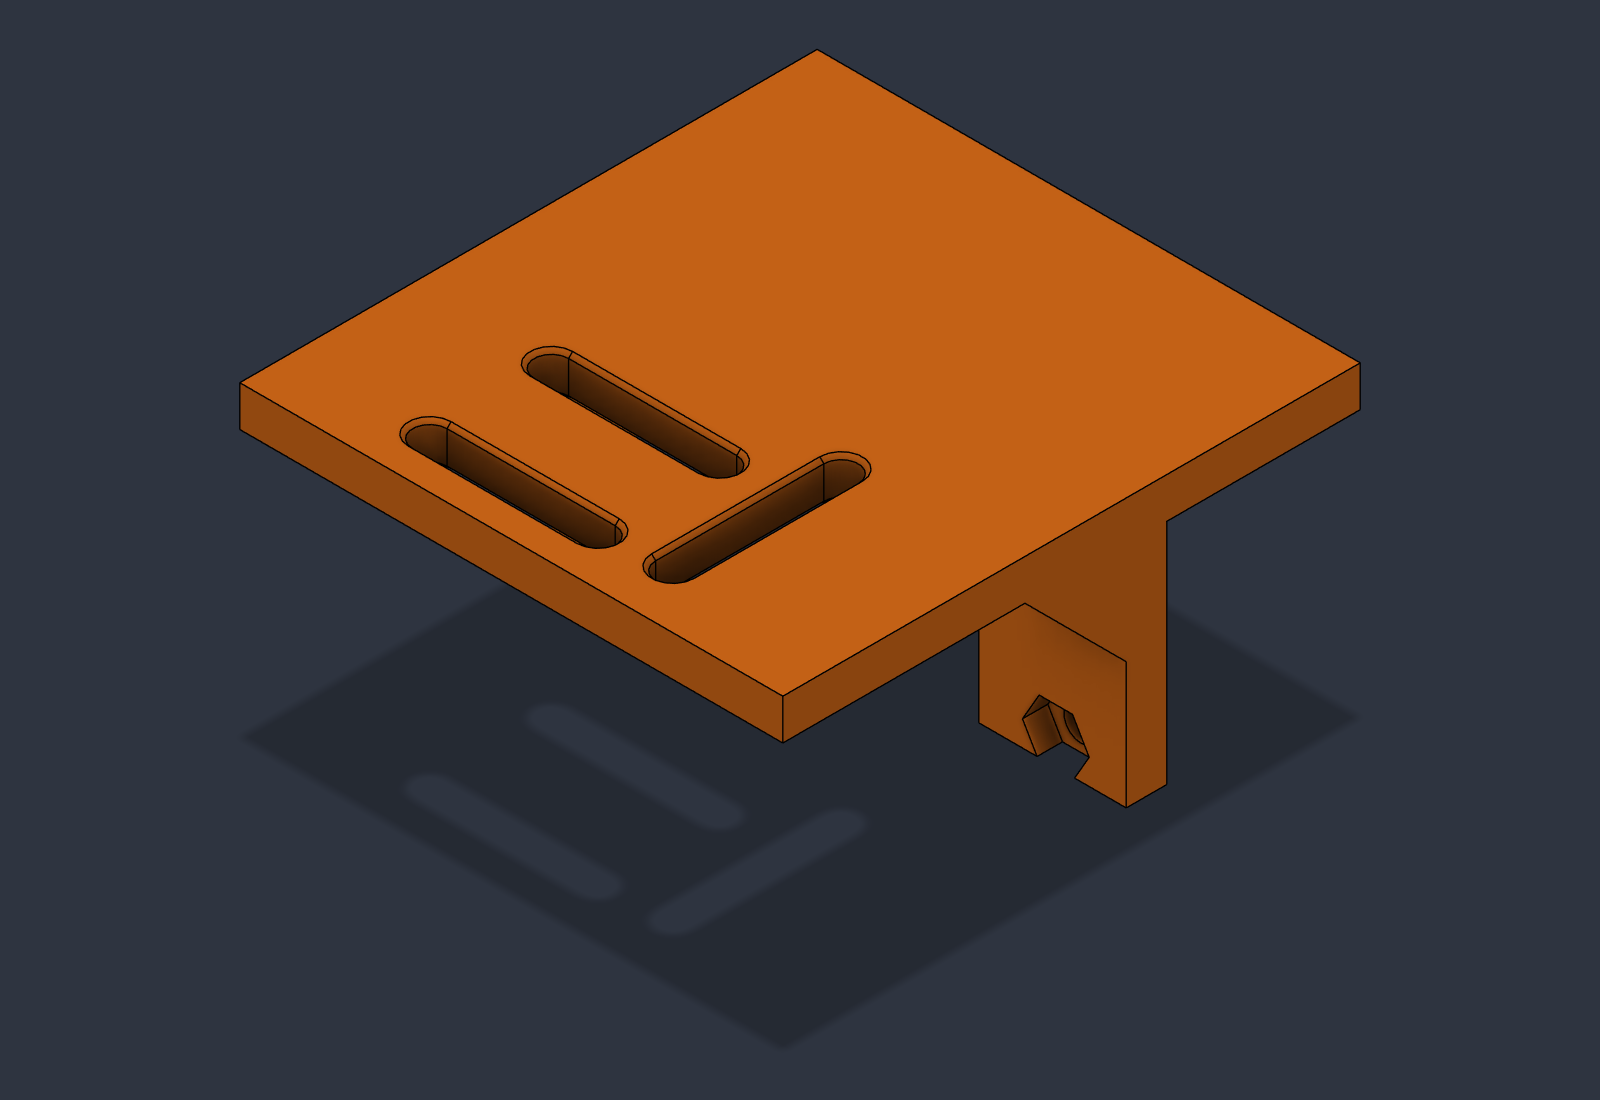
\includegraphics[width=0.48\textwidth]{angle_bracket_iso_rear.png}\\[1ex]
  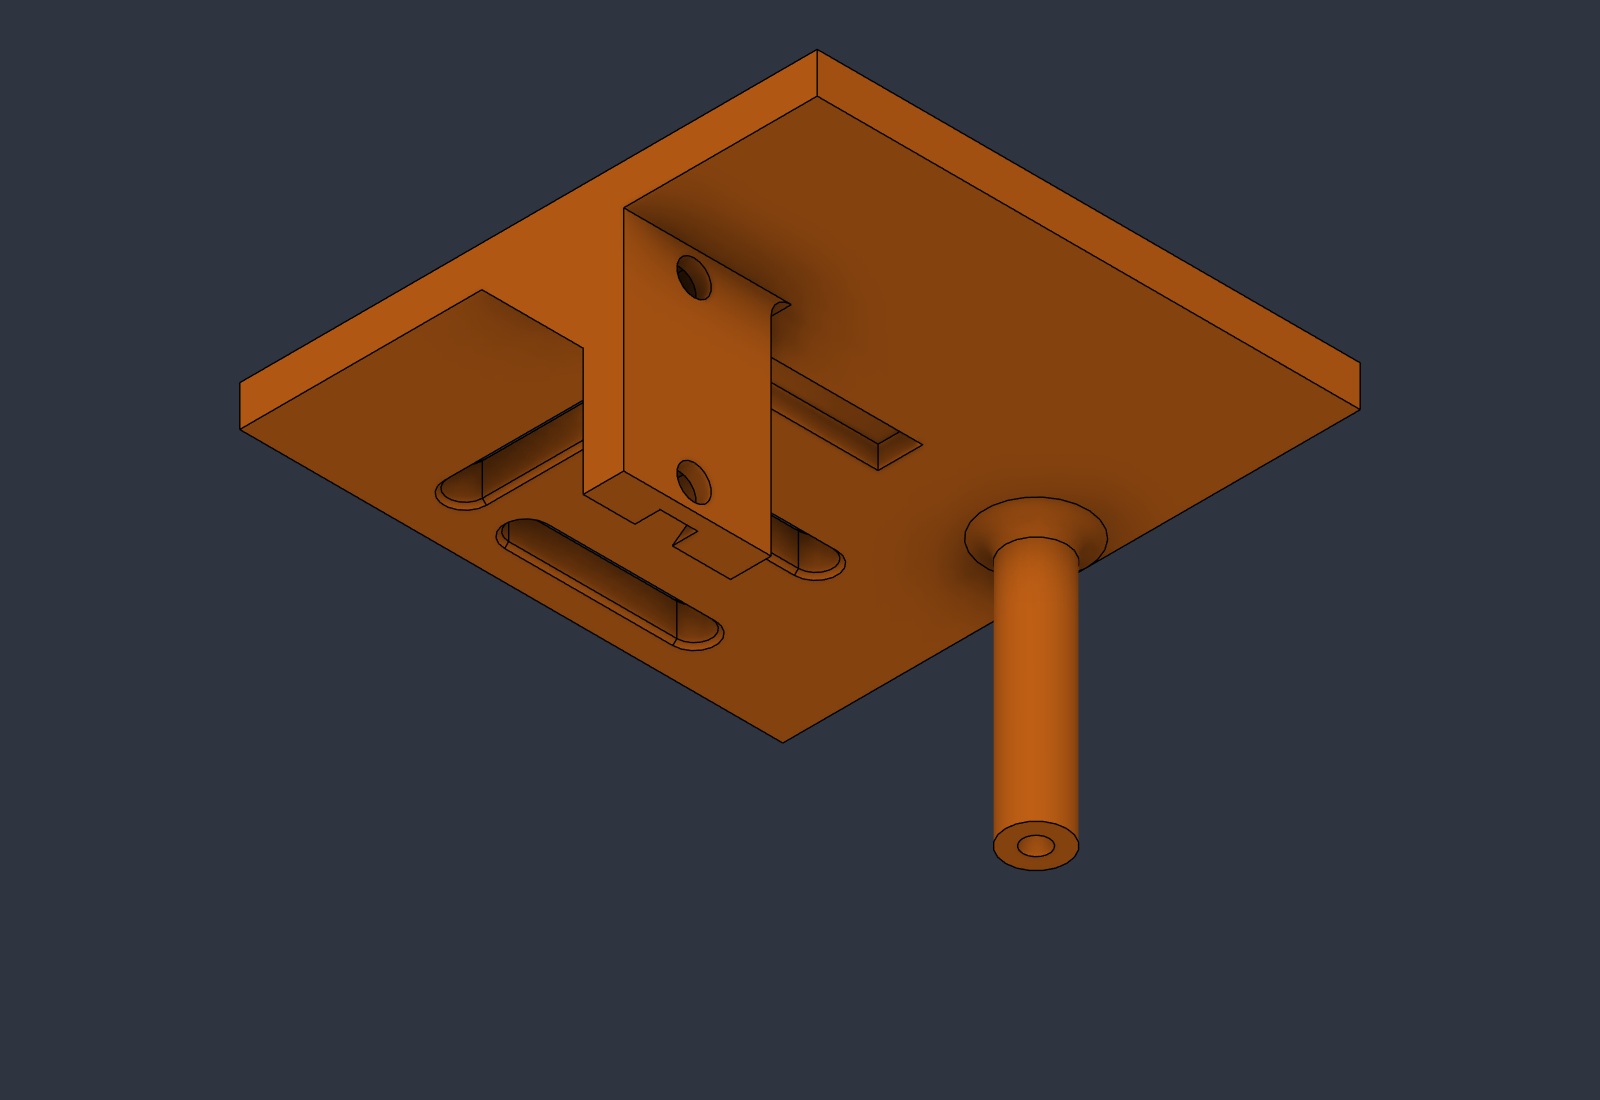
\includegraphics[width=0.48\textwidth]{angle_bracket_under_front.png}\hfill
  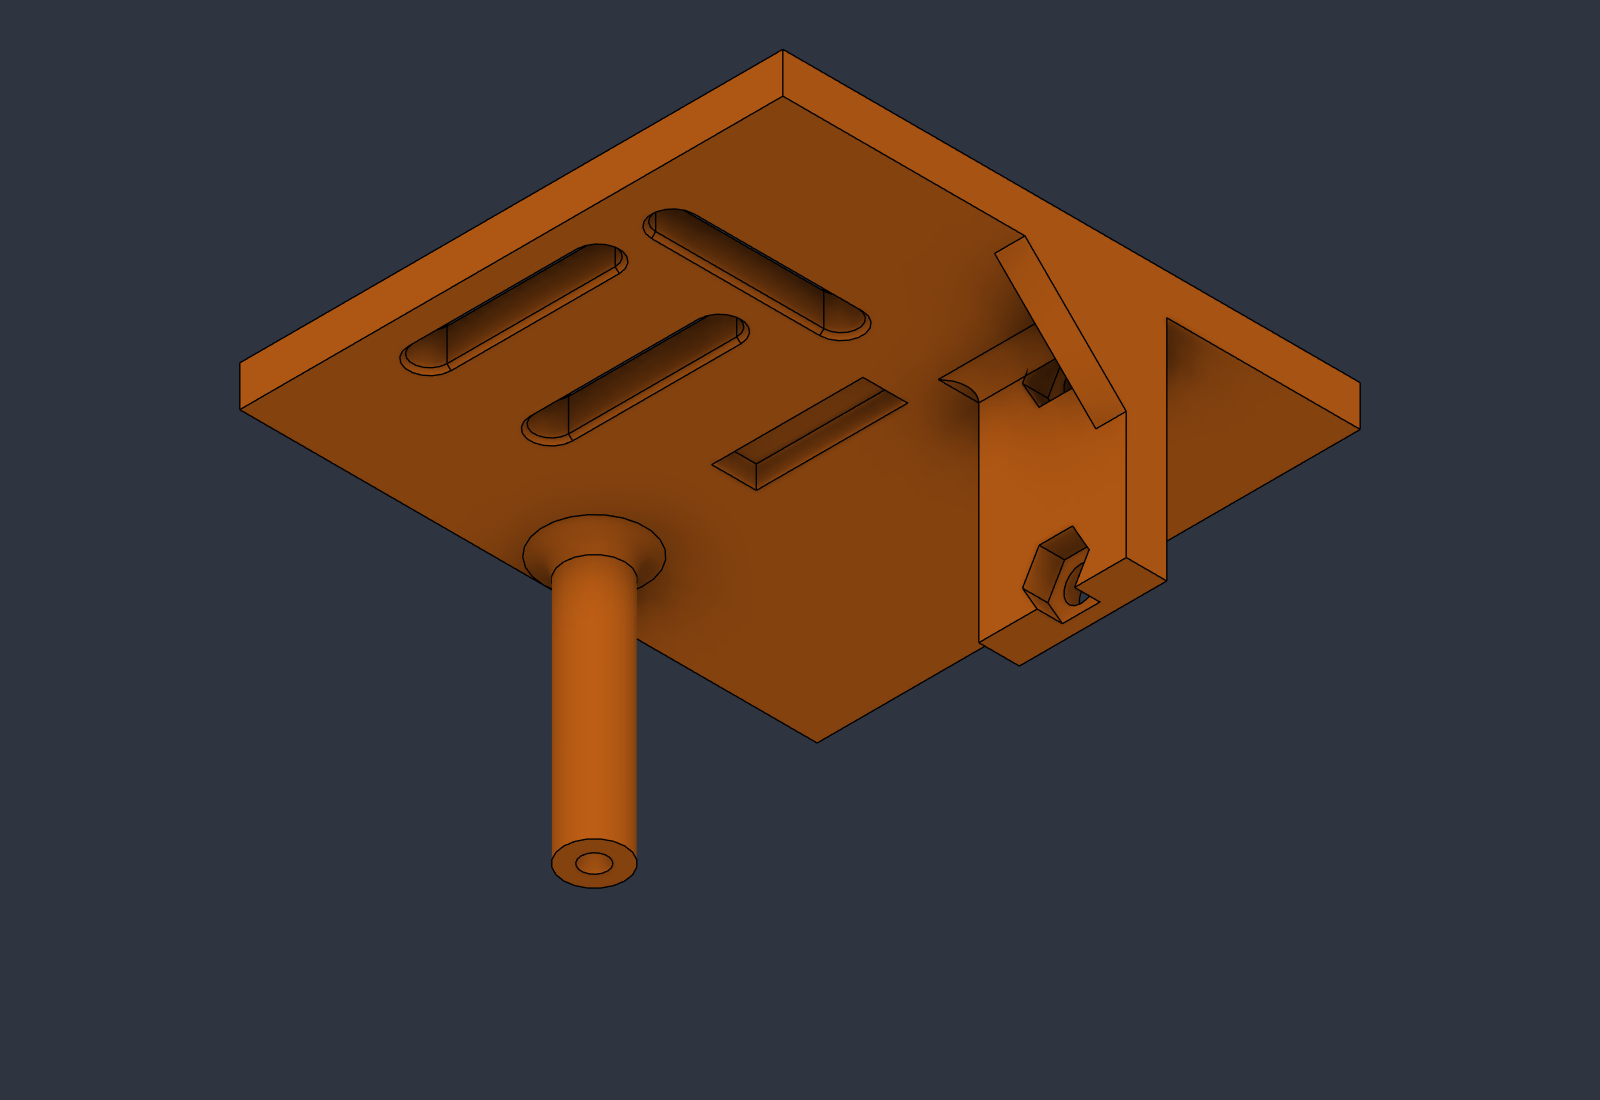
\includegraphics[width=0.48\textwidth]{angle_bracket_under_rear.png}
  \caption{Right bracket on its own: top and underside, from the front and the rear.}
  \label{fig:bracket-angles}
\end{figure}

% F11-F12 -- bracket with motor, disc and LM393 (no wheel, no plate), from below
\begin{figure}[htbp]
  \centering
  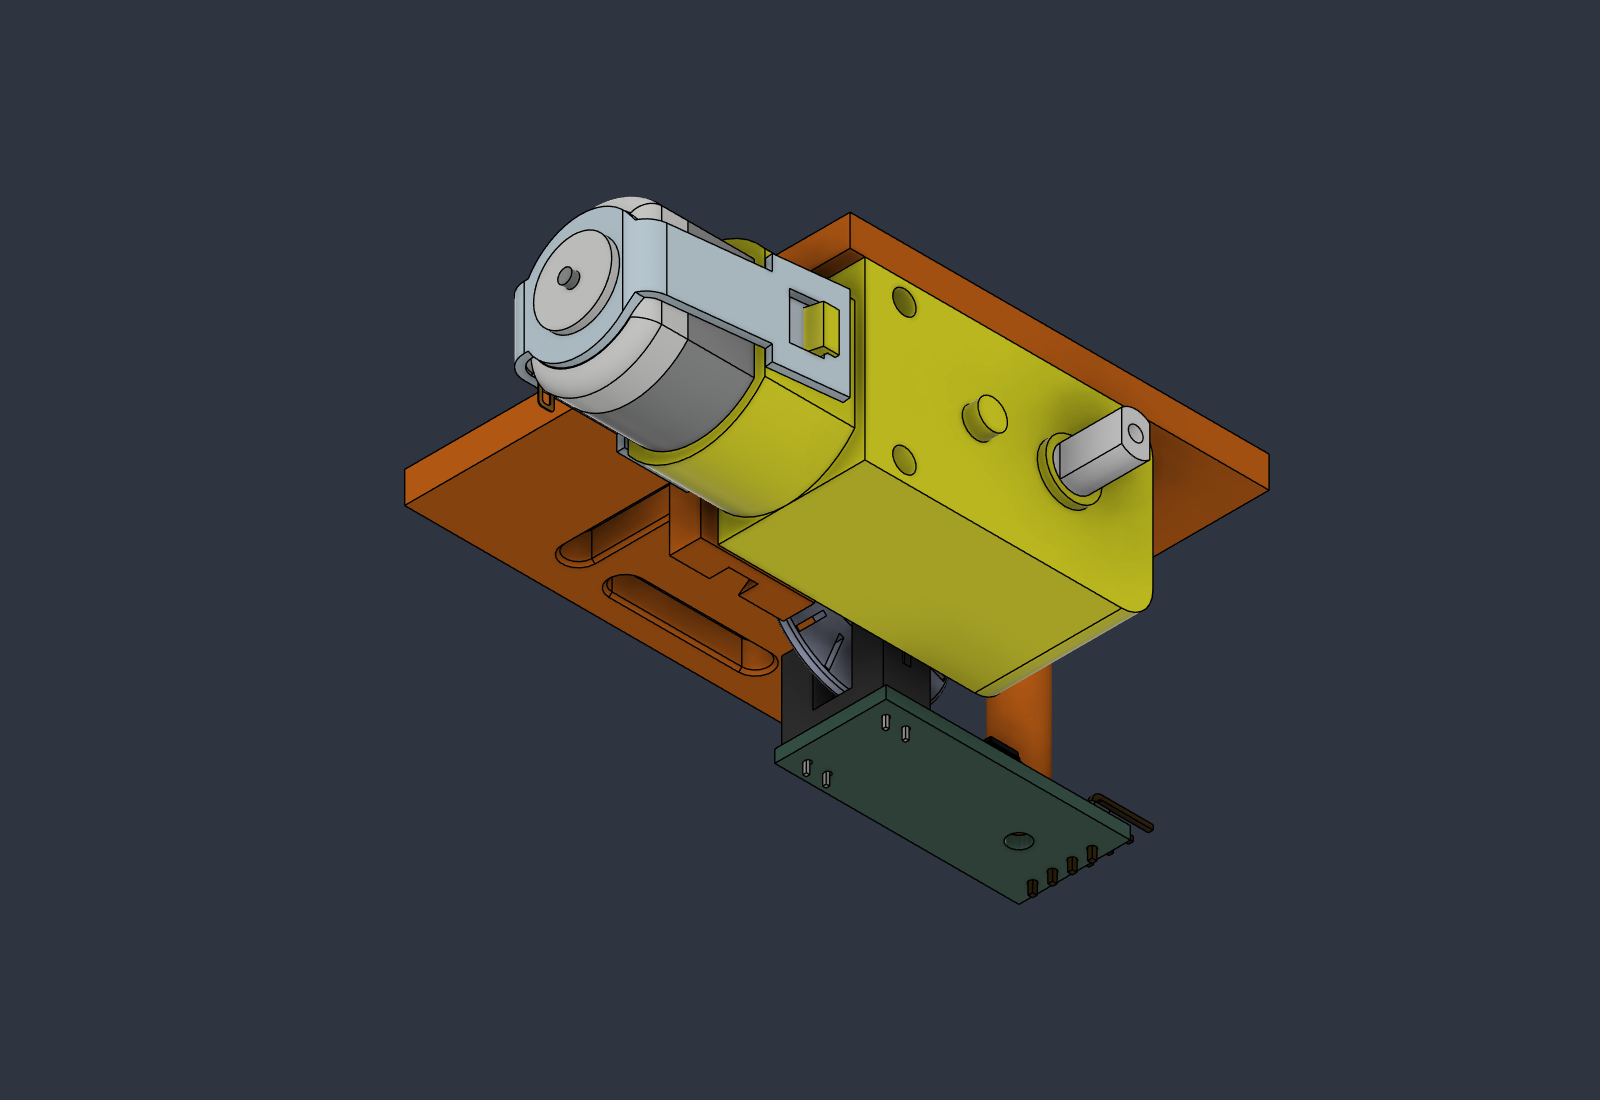
\includegraphics[width=0.48\textwidth]{angle_assembly_under_front.png}\hfill
  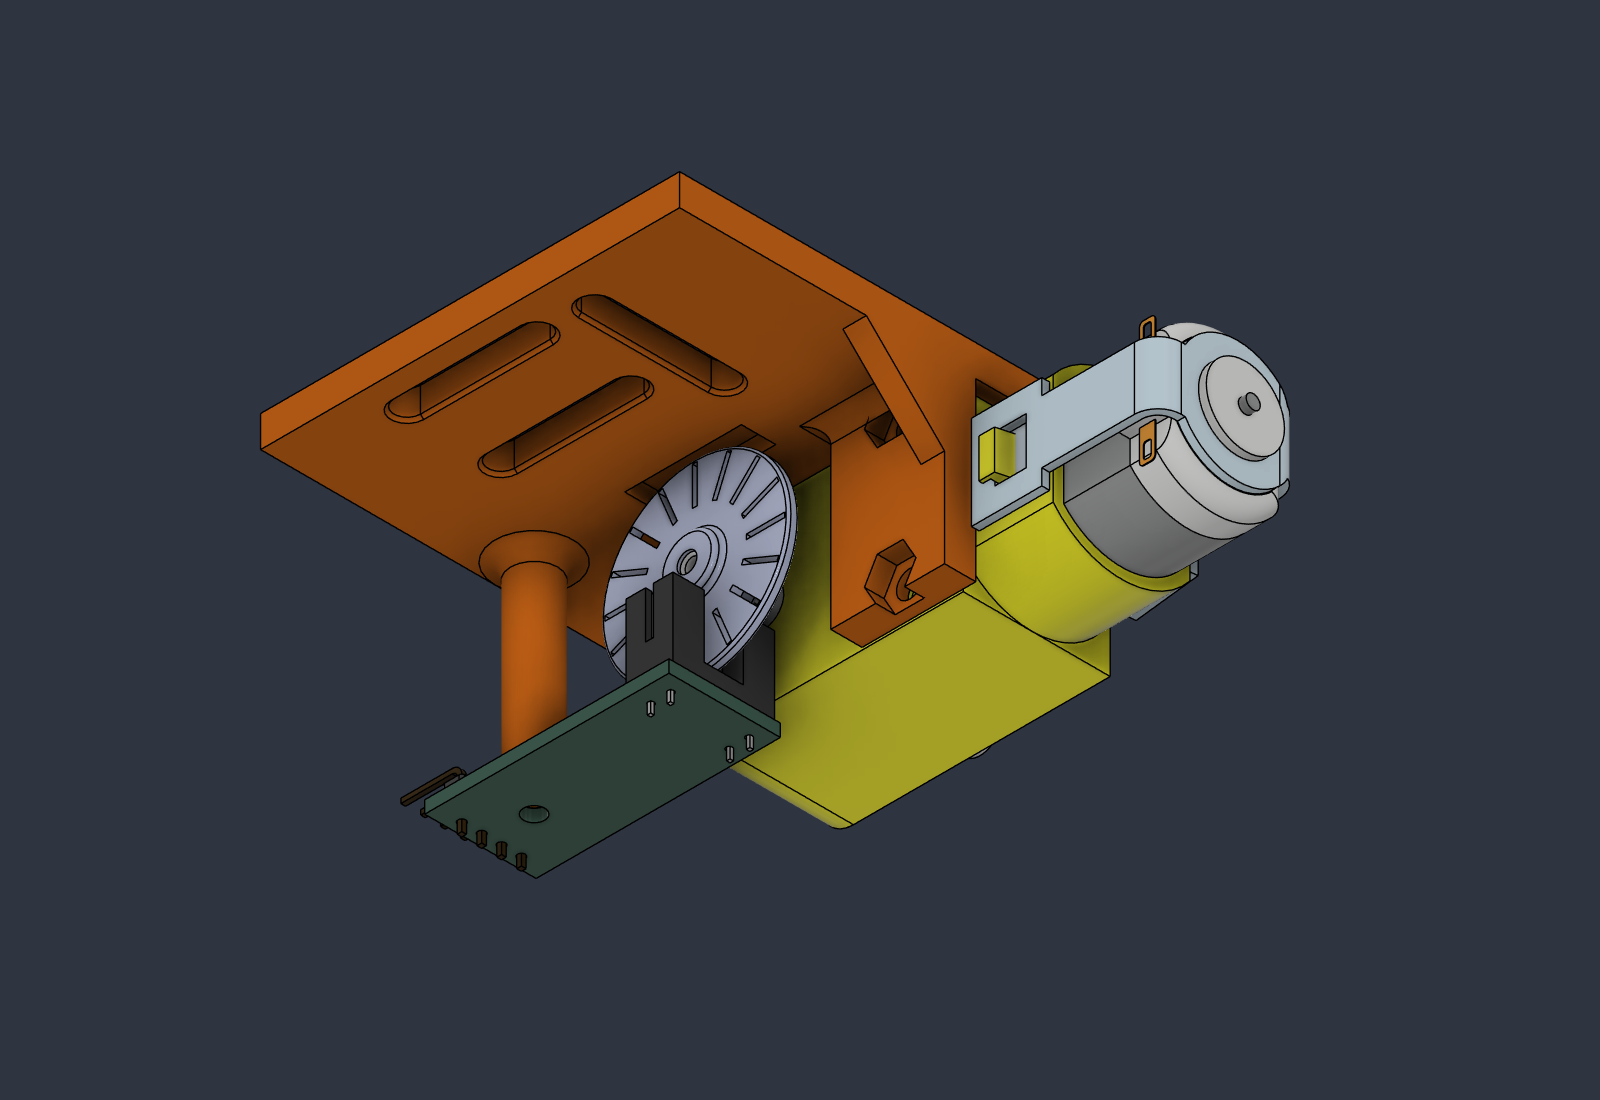
\includegraphics[width=0.48\textwidth]{angle_assembly_under_rear.png}
  \caption{Assembly from below: motor tab and nut traps, encoder disc and LM393 sensor.}
  \label{fig:assembly-below}
\end{figure}
 where needed, or copy single blocks.
% Images live in ../CAD/out/ (see \graphicspath in main.tex), so re-rendering them in
% Fusion updates the thesis without copying files.
% Every figure is also registered in tracking/log.md with how it was produced.
% Naming: label fig:<topic>-<view>.

% F01 -- made with Fusion viewport.saveAsImageFile, iso top-right view, plate hidden
\begin{figure}[htbp]
  \centering
  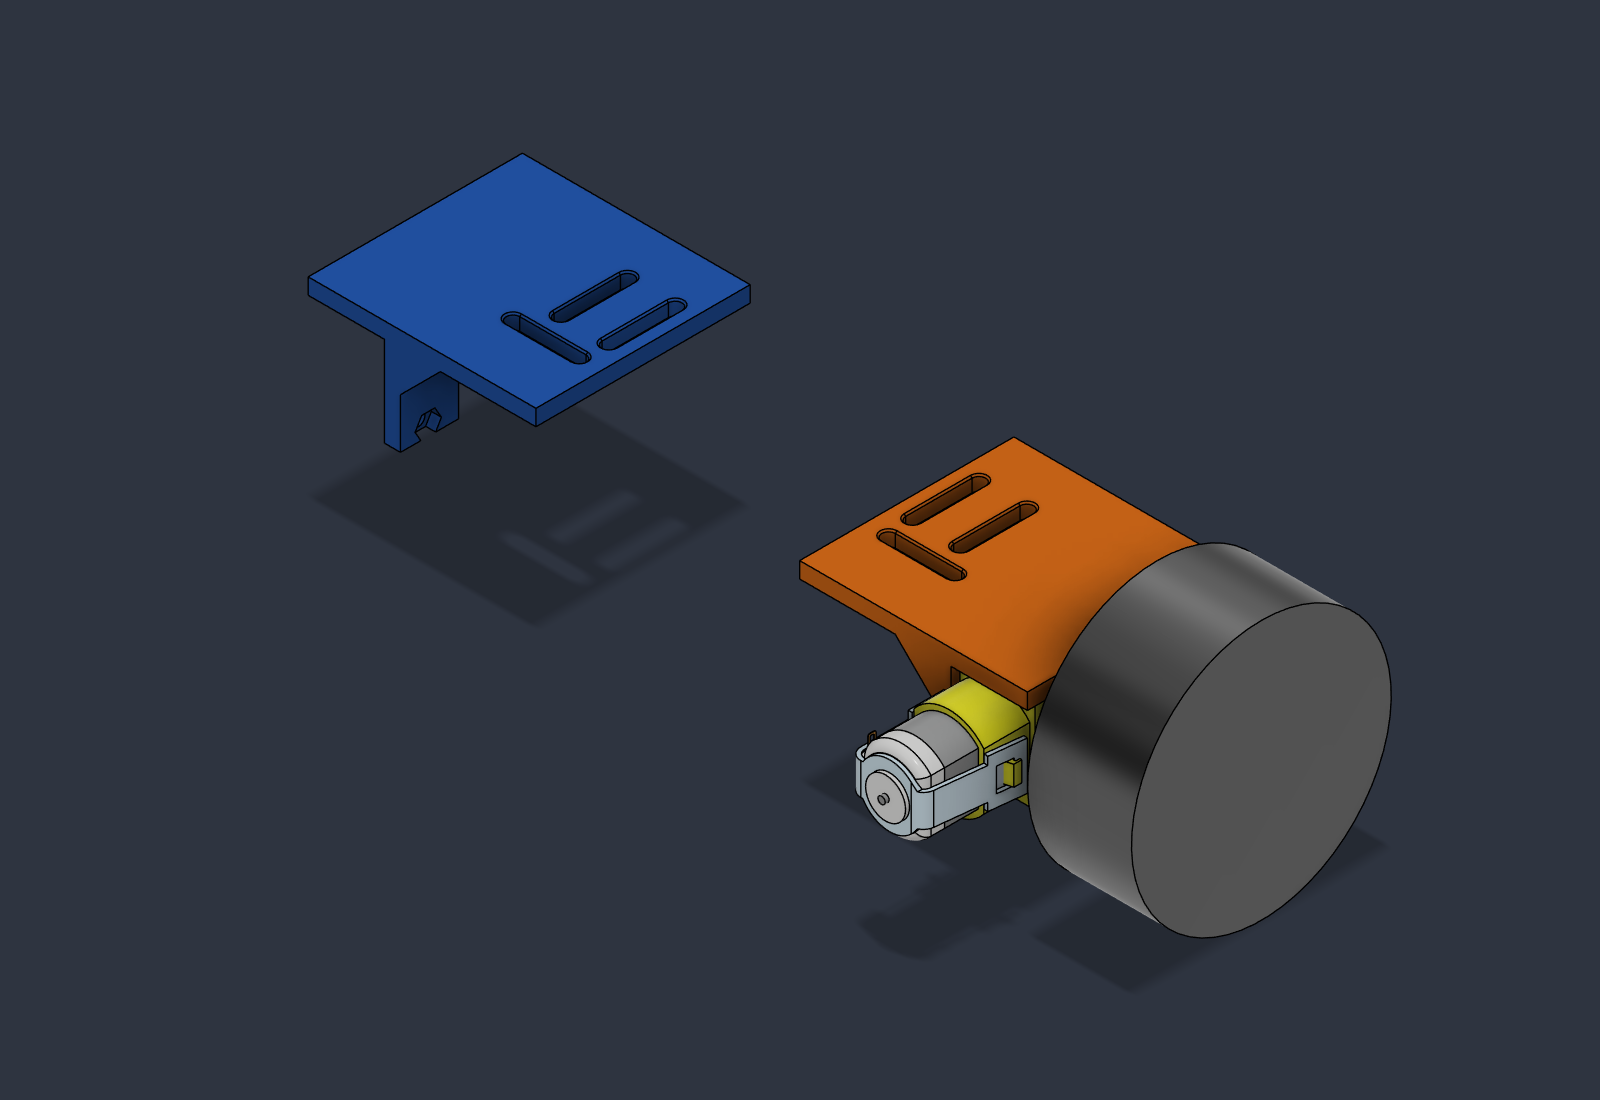
\includegraphics[width=0.85\textwidth]{shot_iso.png}
  \caption{Right and left motor brackets with the right-hand TT motor and wheel
           (isometric view).}
  \label{fig:bracket-iso}
\end{figure}

% F02 -- top view, plate hidden
\begin{figure}[htbp]
  \centering
  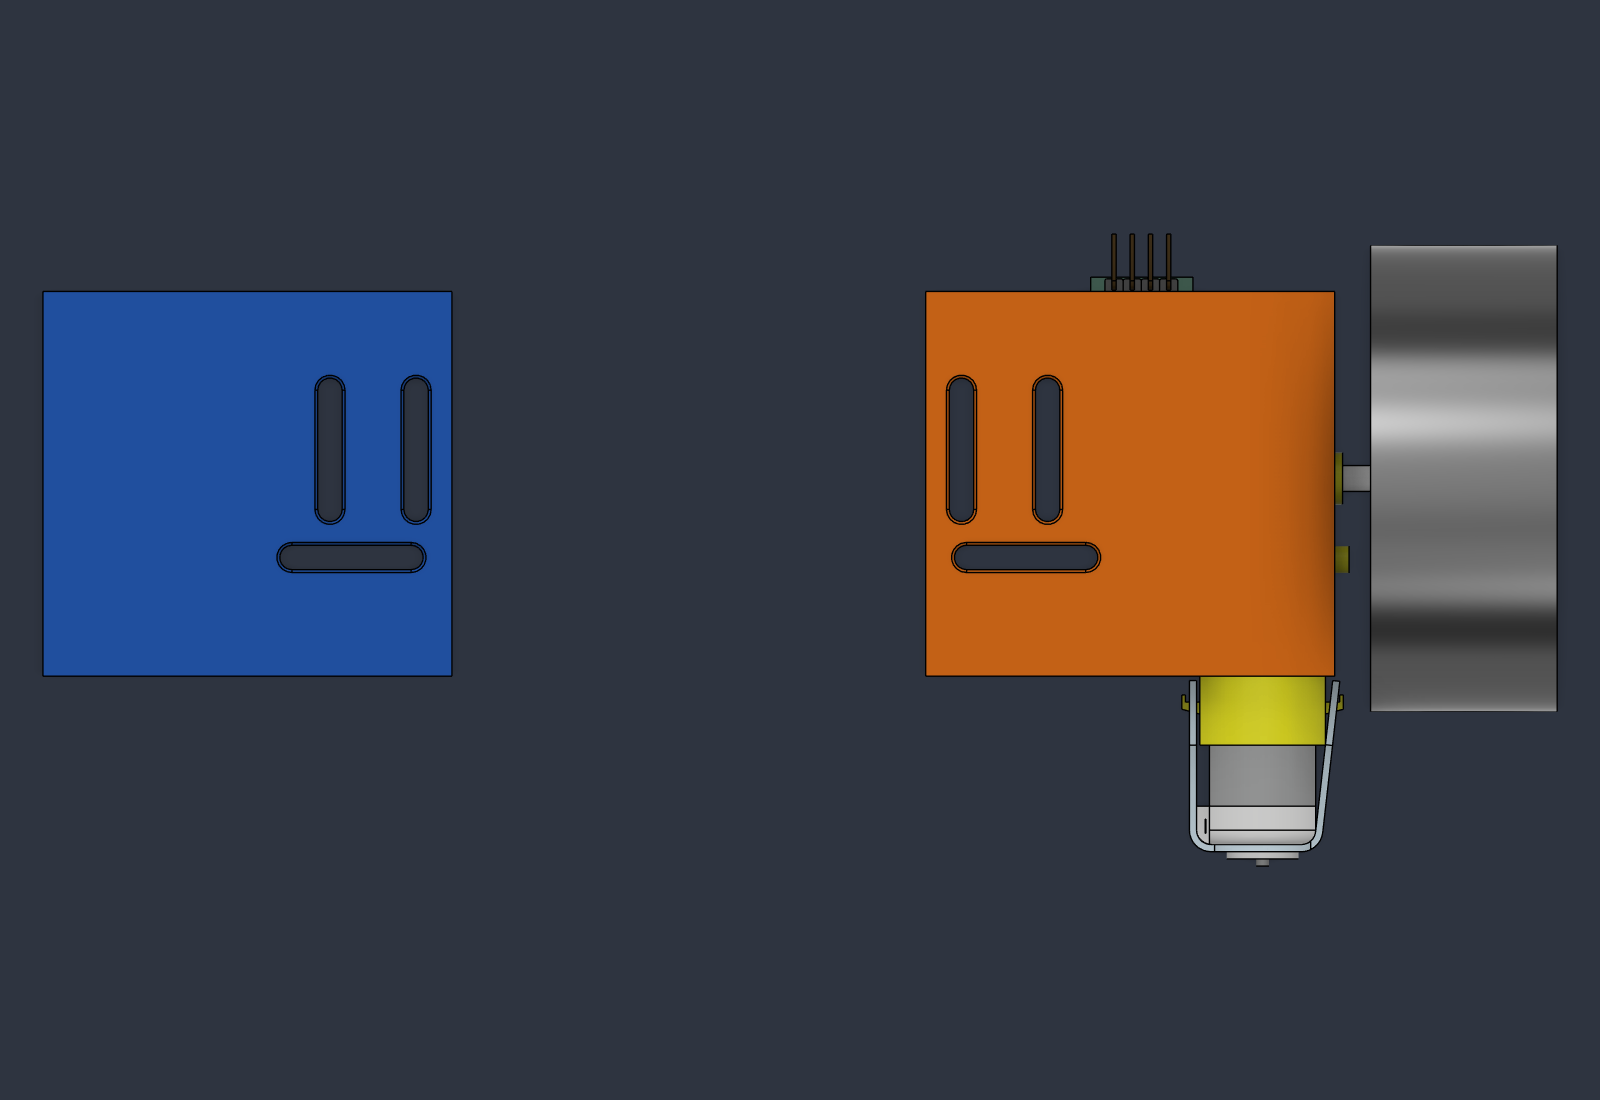
\includegraphics[width=0.85\textwidth]{shot_top.png}
  \caption{Top view of both brackets showing the three mounting slots.}
  \label{fig:bracket-top}
\end{figure}

% F03 -- Fusion "front" view (looks along +Y), plate hidden
\begin{figure}[htbp]
  \centering
  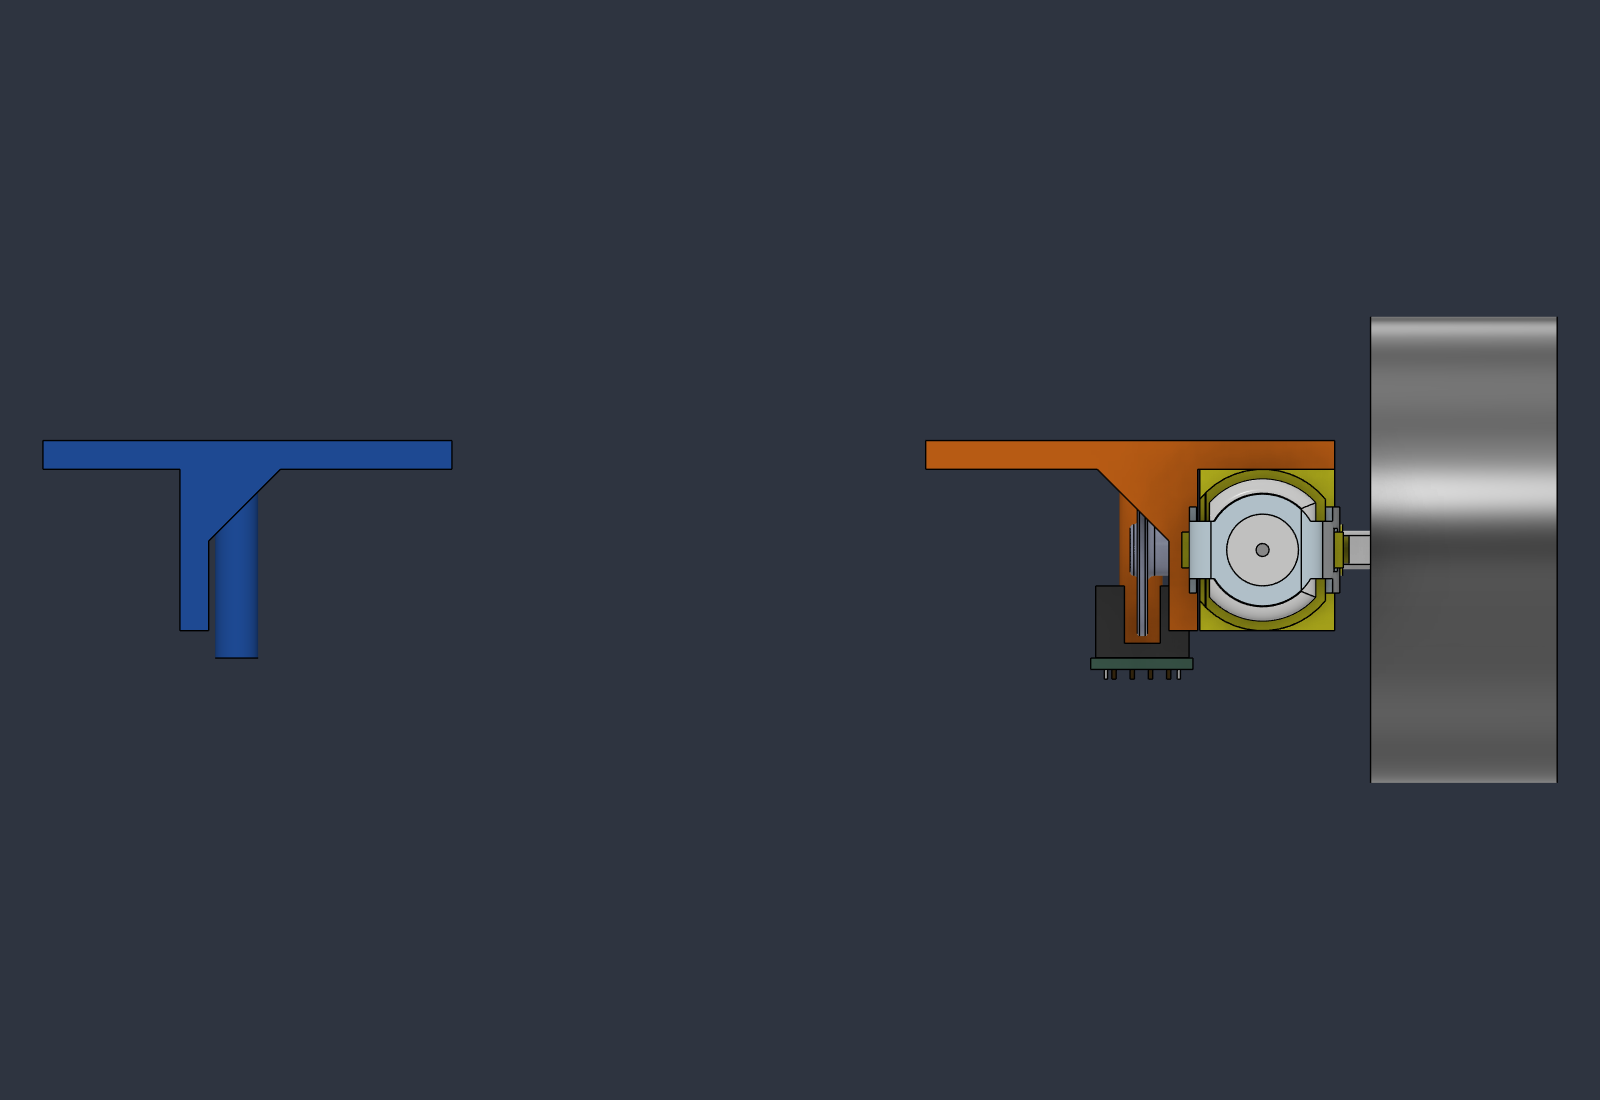
\includegraphics[width=0.85\textwidth]{shot_front.png}
  \caption{Front view: flange on the gearbox top, motor tab and sensor column.}
  \label{fig:bracket-front}
\end{figure}

% F04 -- left view, plate, wheel and left bracket hidden
\begin{figure}[htbp]
  \centering
  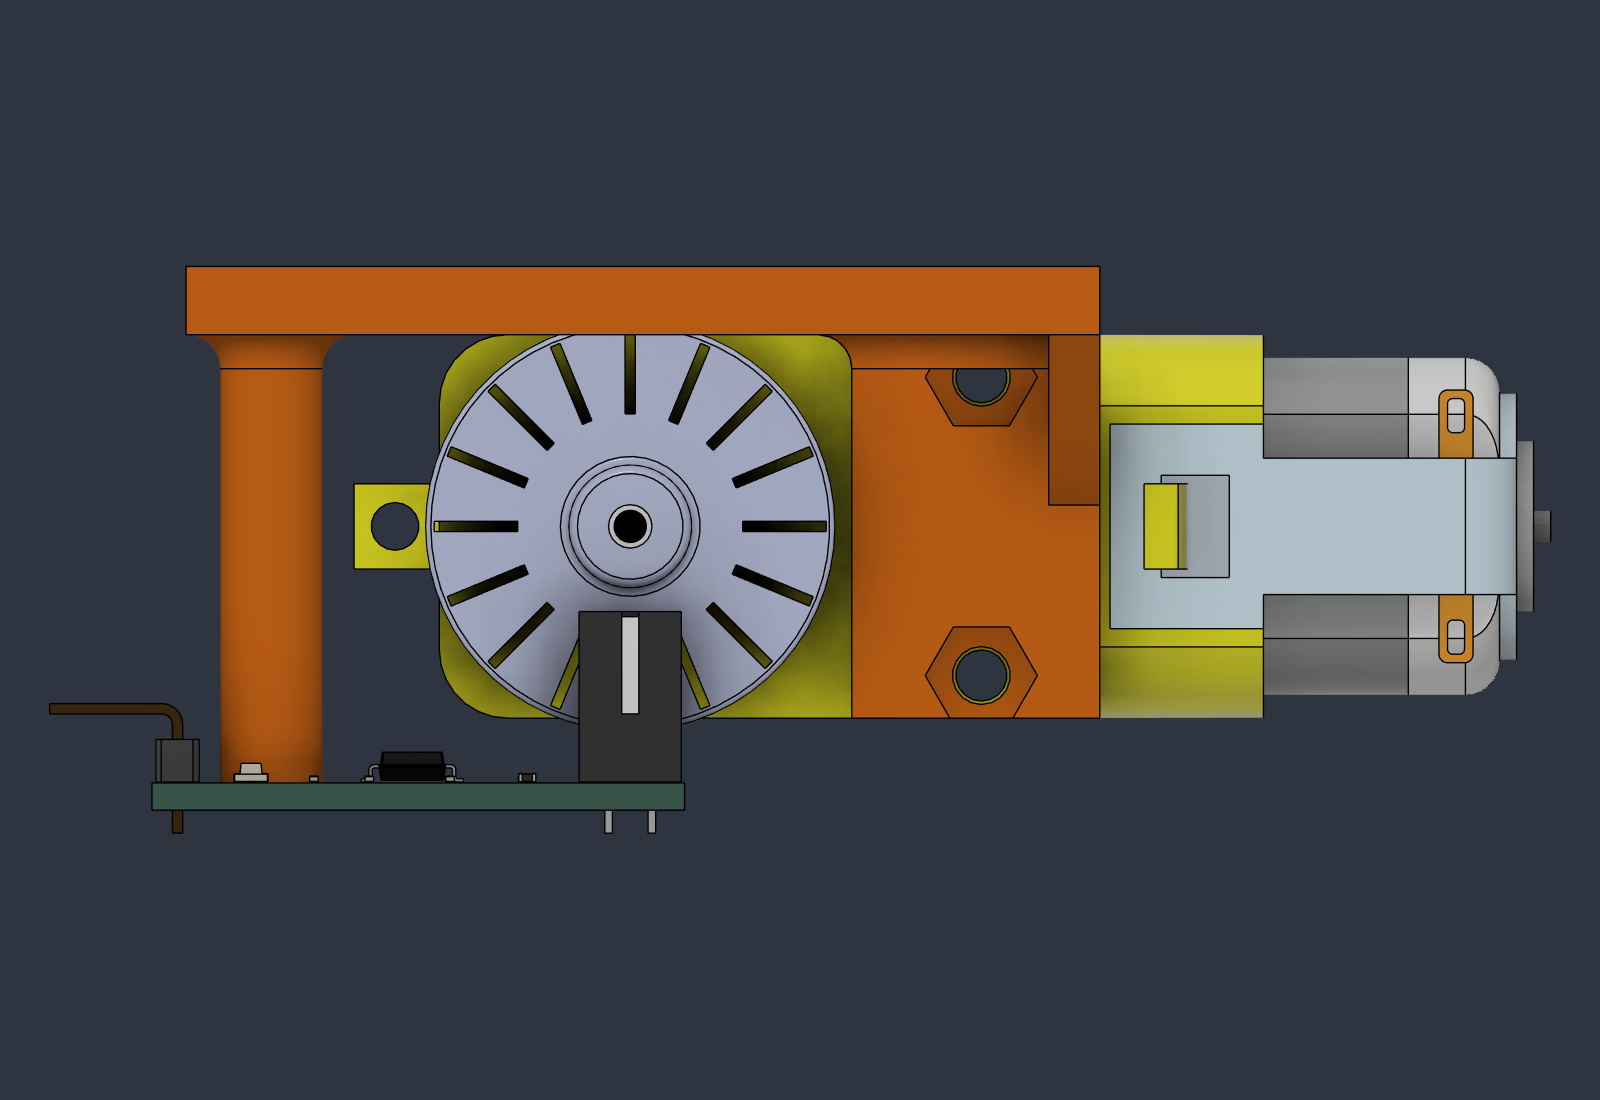
\includegraphics[width=0.85\textwidth]{shot_side.png}
  \caption{Side view: the encoder disc's bottom rim sits in the LM393 fork; the board is
           screwed to the column.}
  \label{fig:sensor-side}
\end{figure}

% F05 -- iso bottom-right view, plate shown
\begin{figure}[htbp]
  \centering
  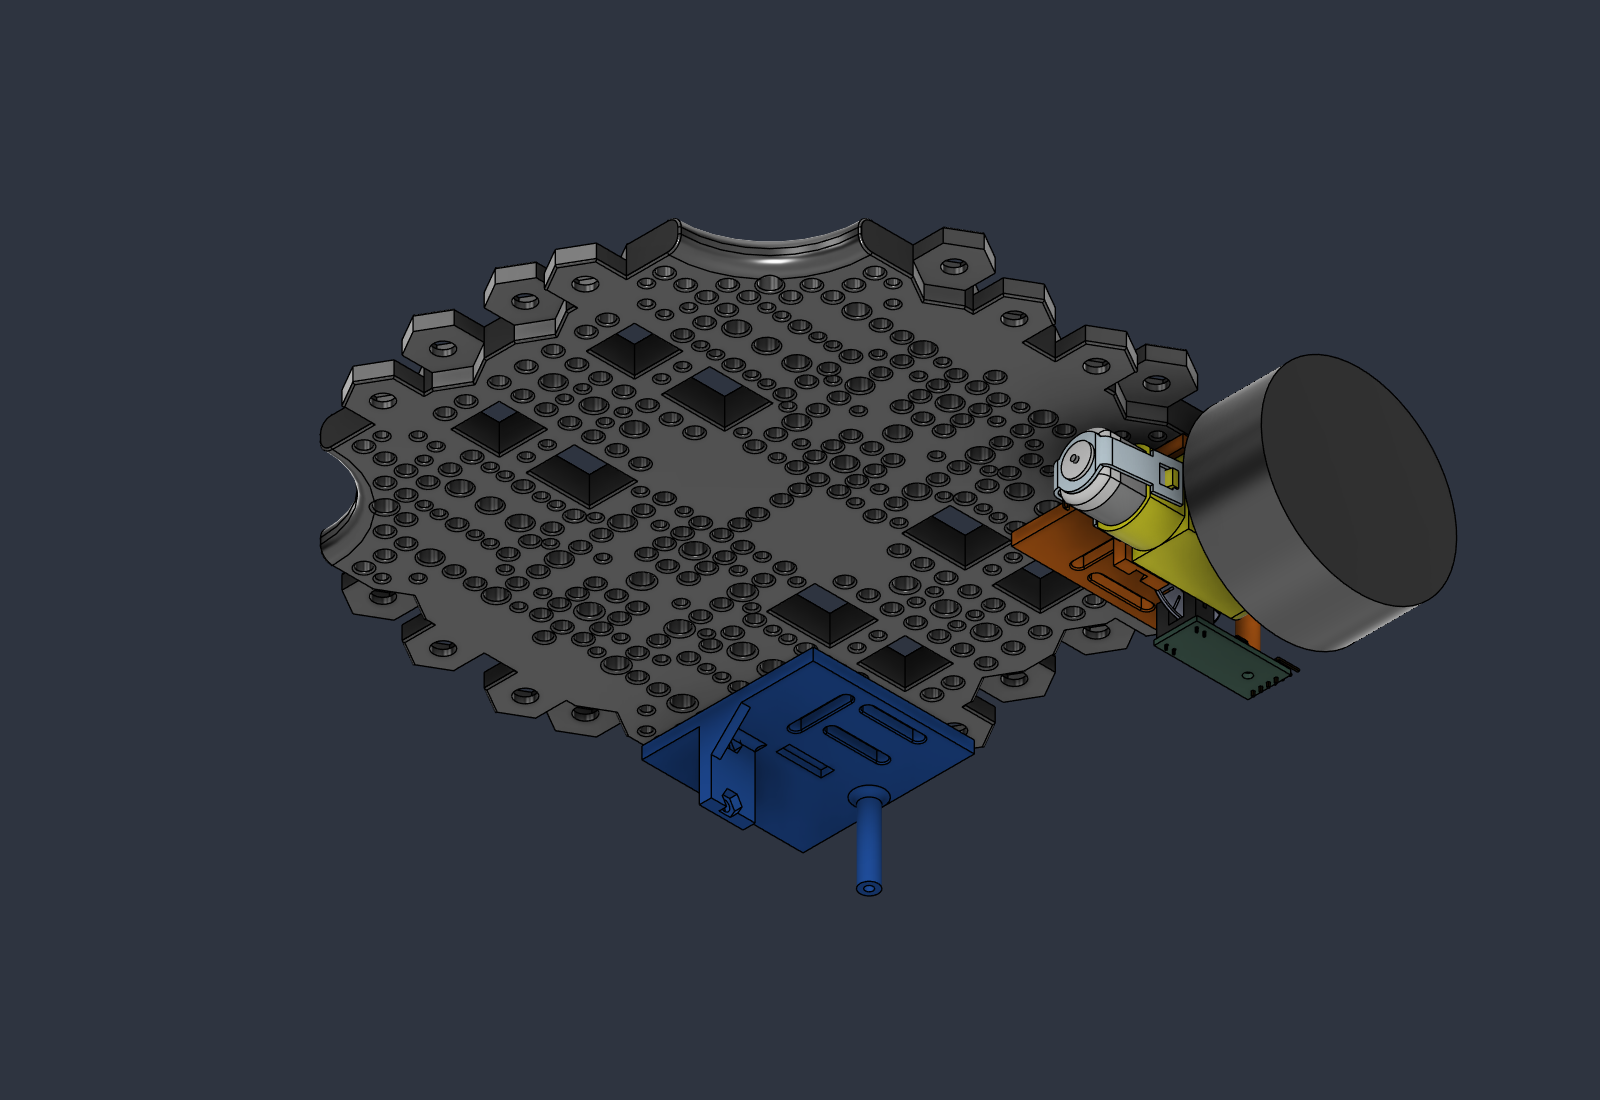
\includegraphics[width=0.85\textwidth]{shot_with_plate_below.png}
  \caption{Brackets mounted under the waffle plate, seen from below.}
  \label{fig:plate-below}
\end{figure}

% F06 -- iso top-right view, plate shown
\begin{figure}[htbp]
  \centering
  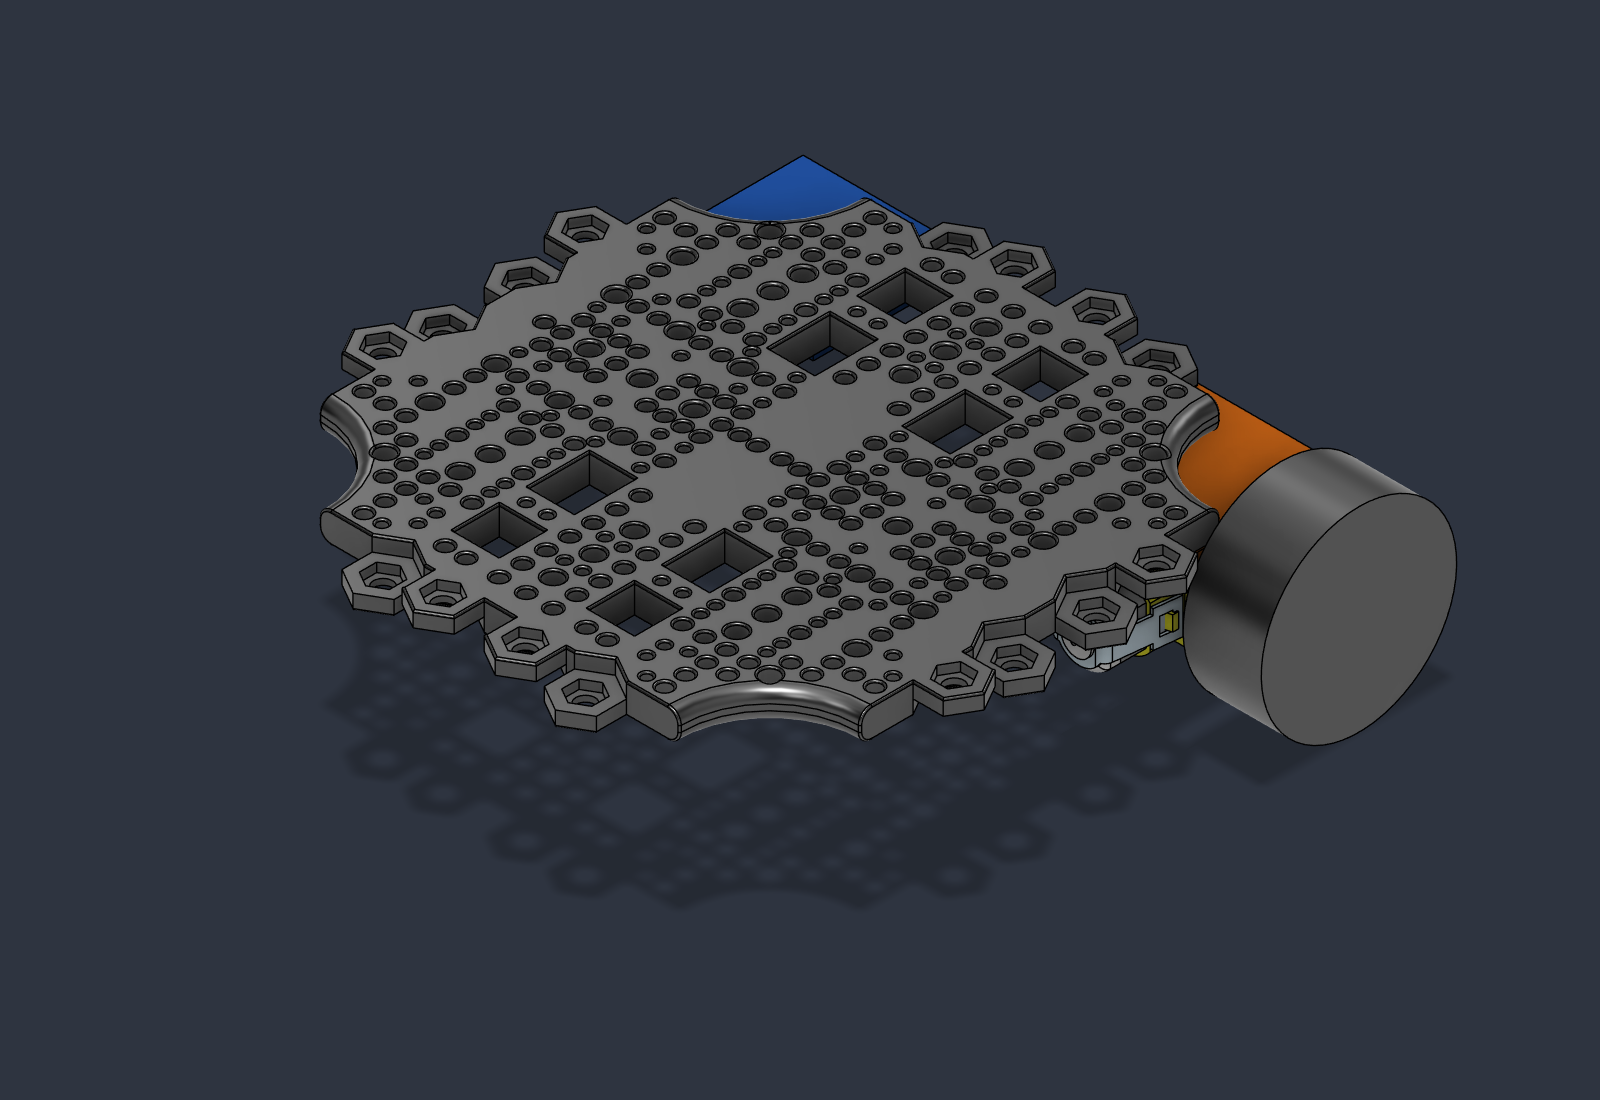
\includegraphics[width=0.85\textwidth]{shot_with_plate_top.png}
  \caption{Brackets and wheel relative to the waffle plate, seen from above.}
  \label{fig:plate-top}
\end{figure}

% F07-F10 -- bracket alone (all references hidden), four isometric views
\begin{figure}[htbp]
  \centering
  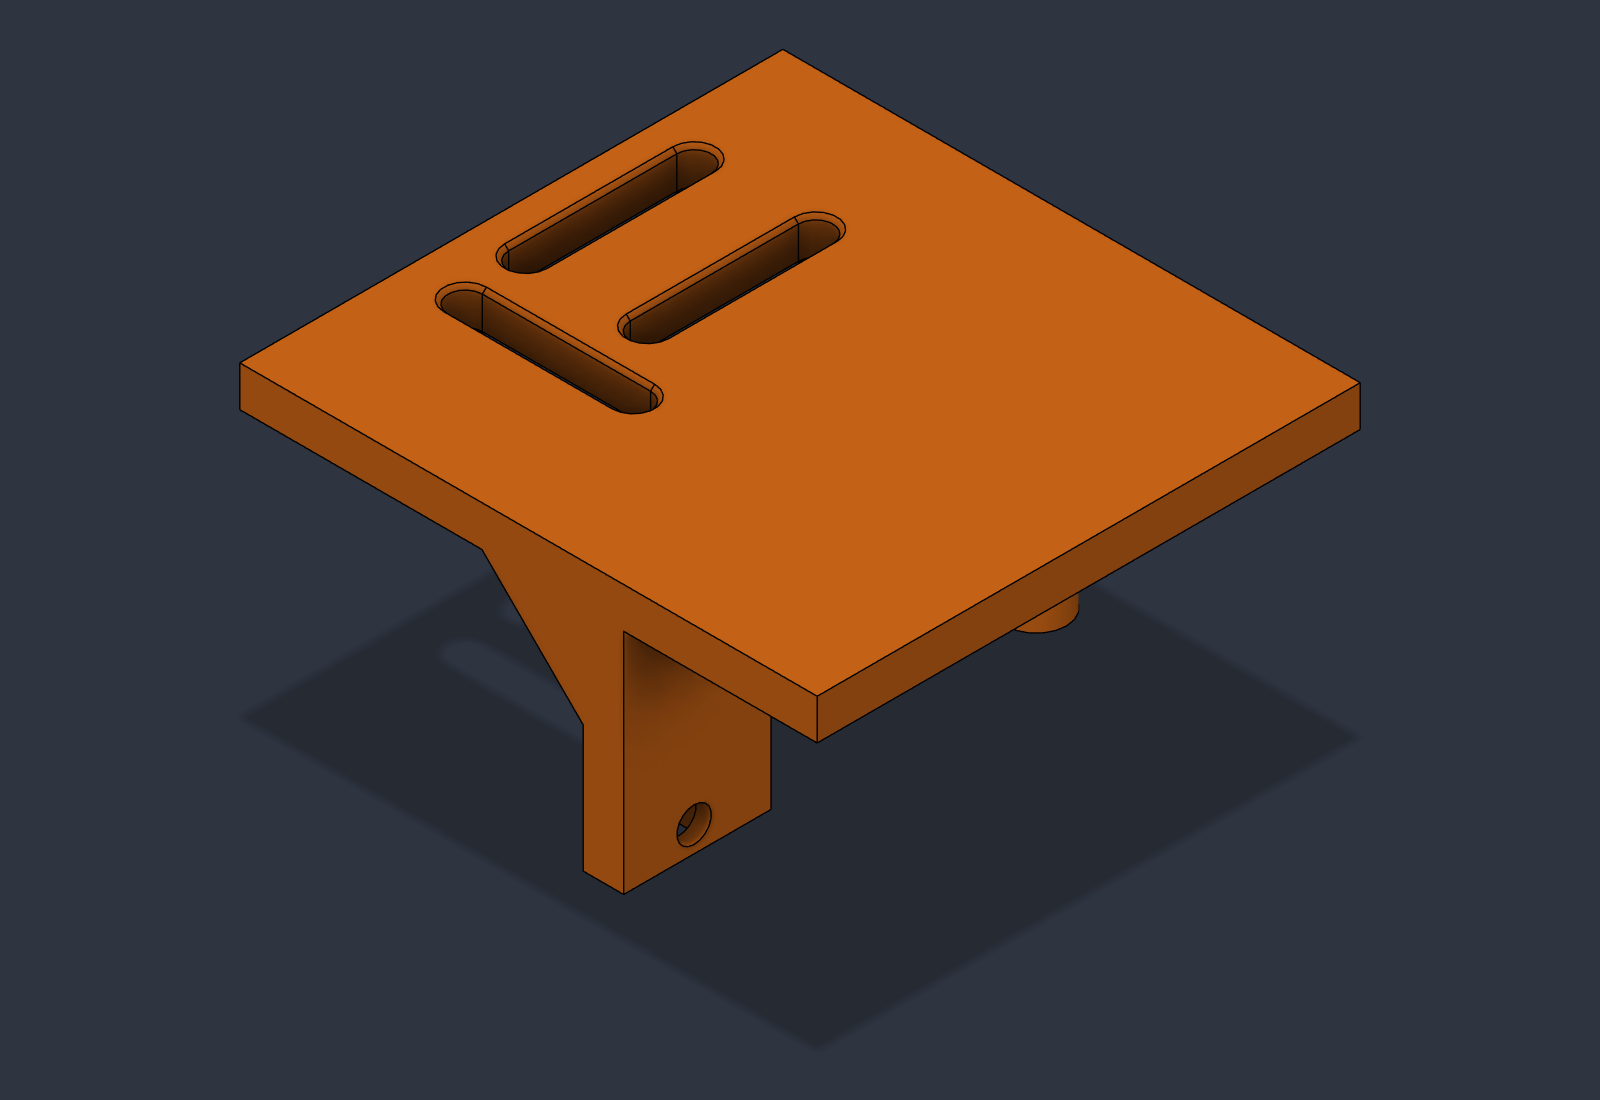
\includegraphics[width=0.48\textwidth]{angle_bracket_iso_front.png}\hfill
  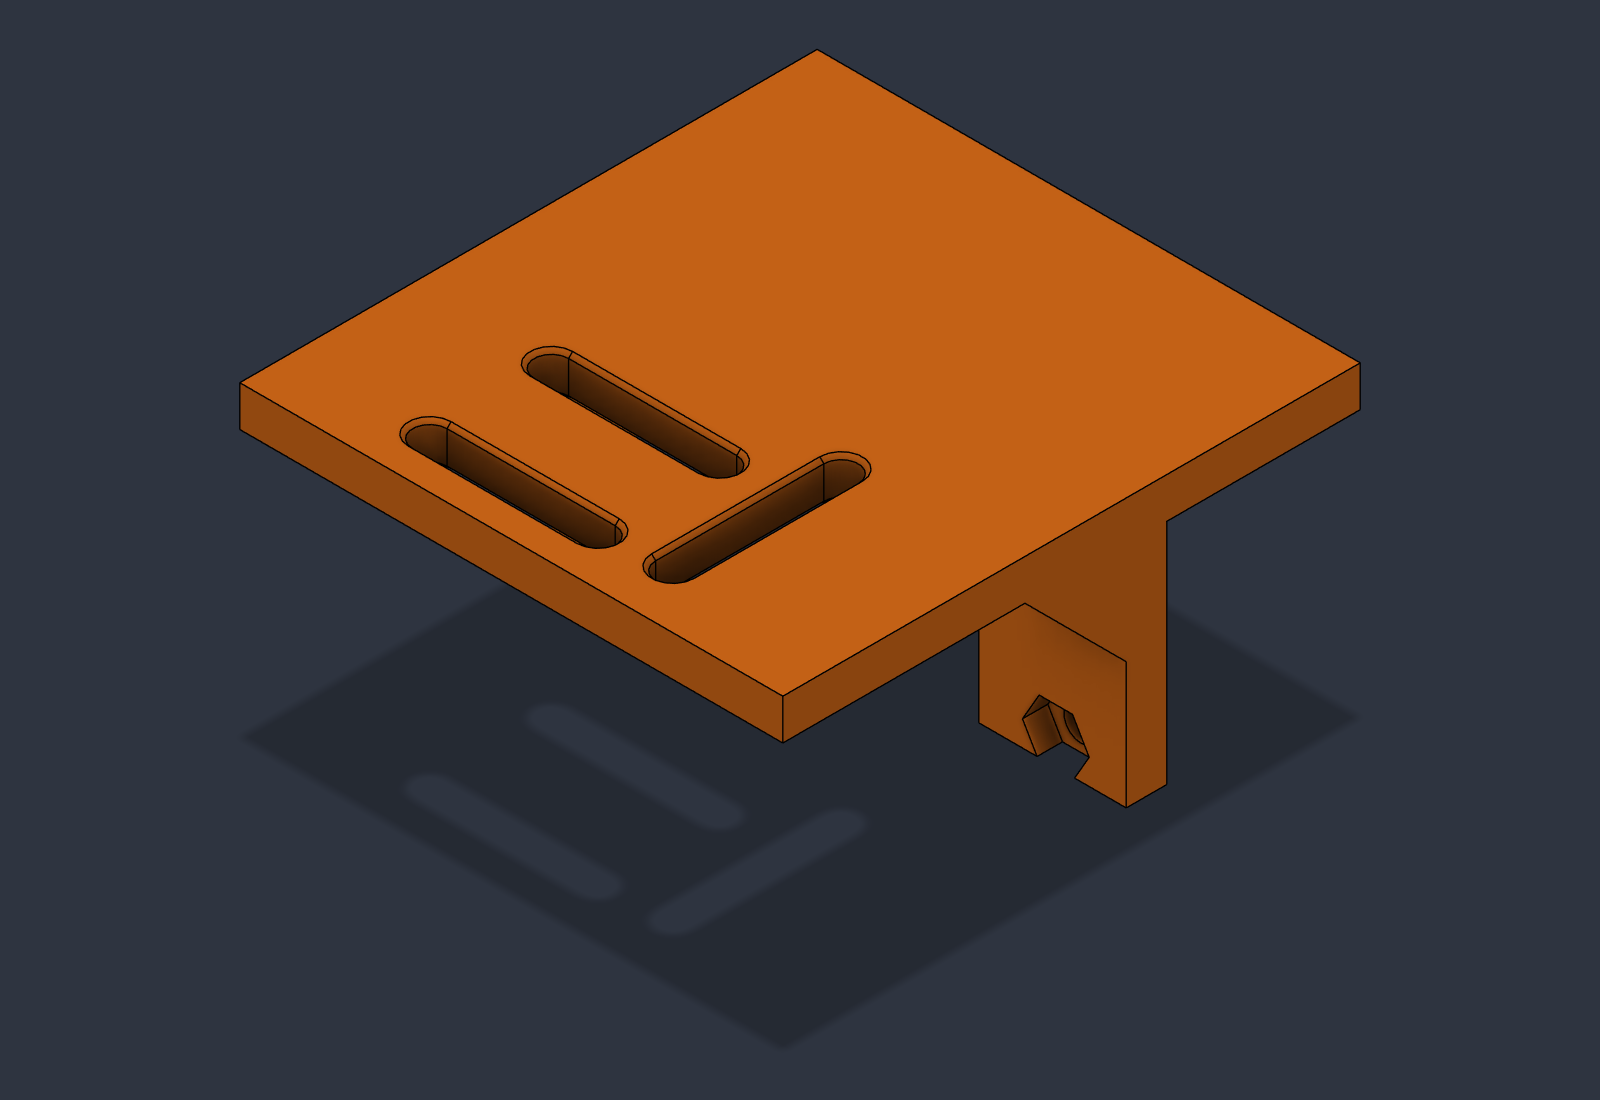
\includegraphics[width=0.48\textwidth]{angle_bracket_iso_rear.png}\\[1ex]
  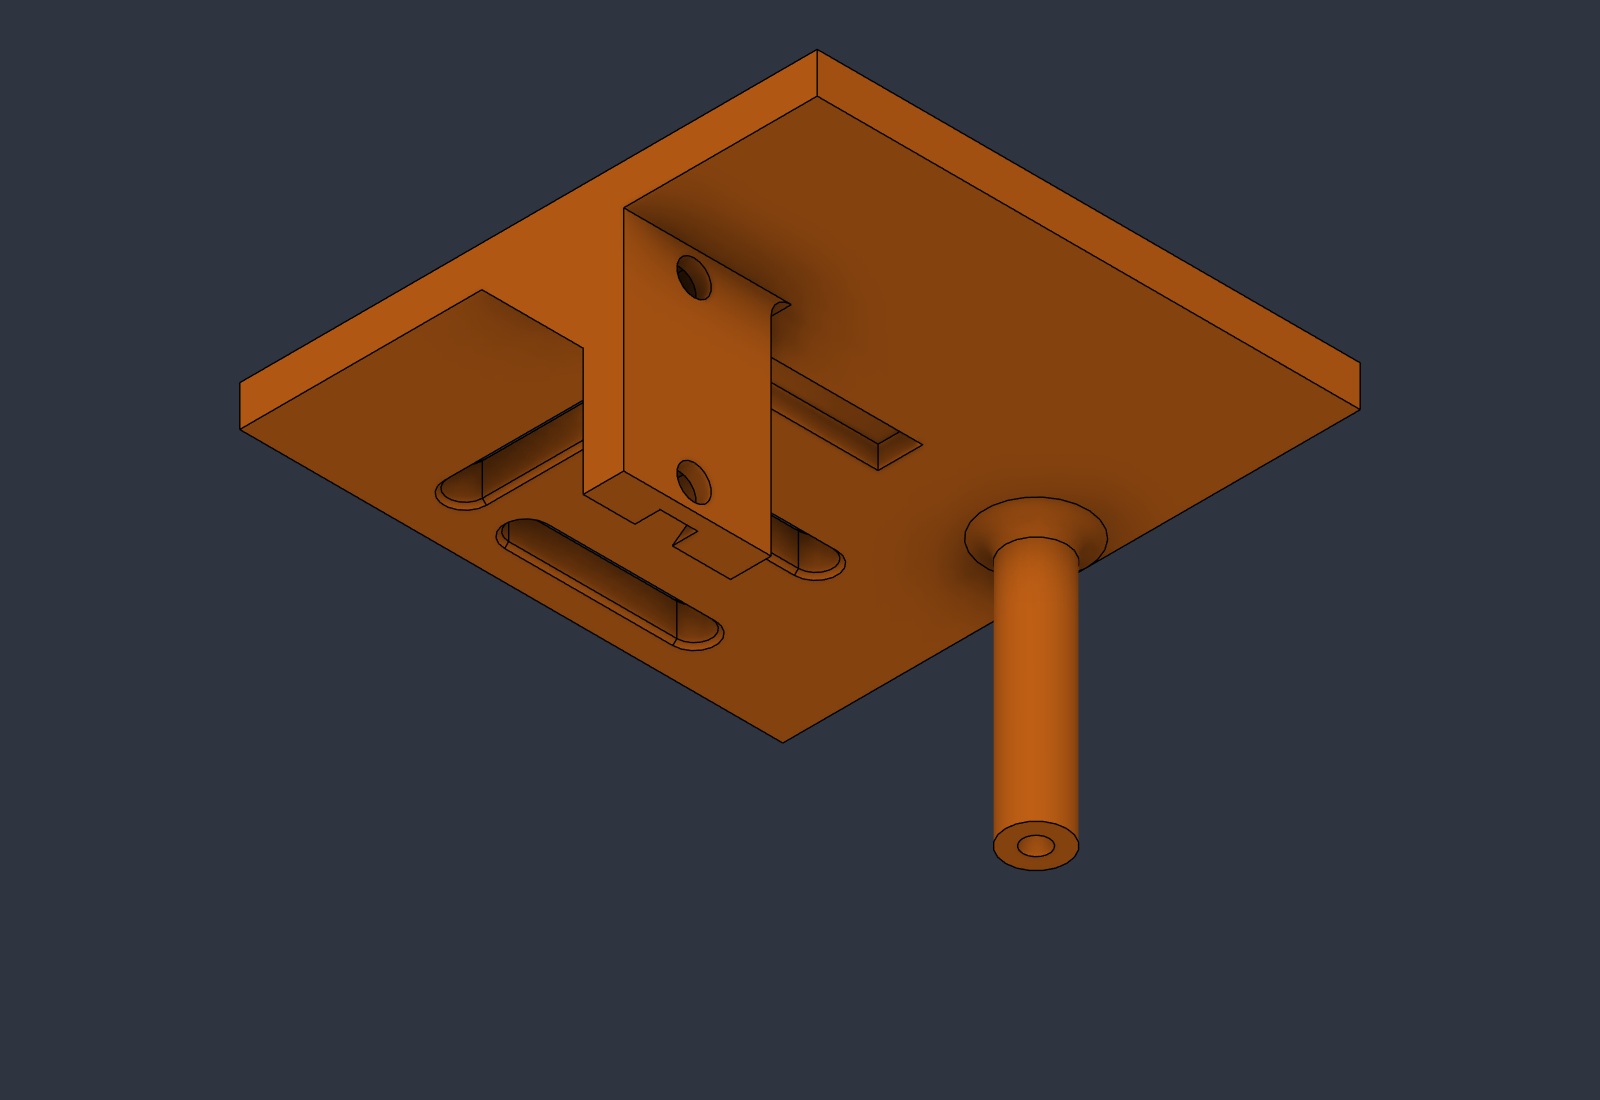
\includegraphics[width=0.48\textwidth]{angle_bracket_under_front.png}\hfill
  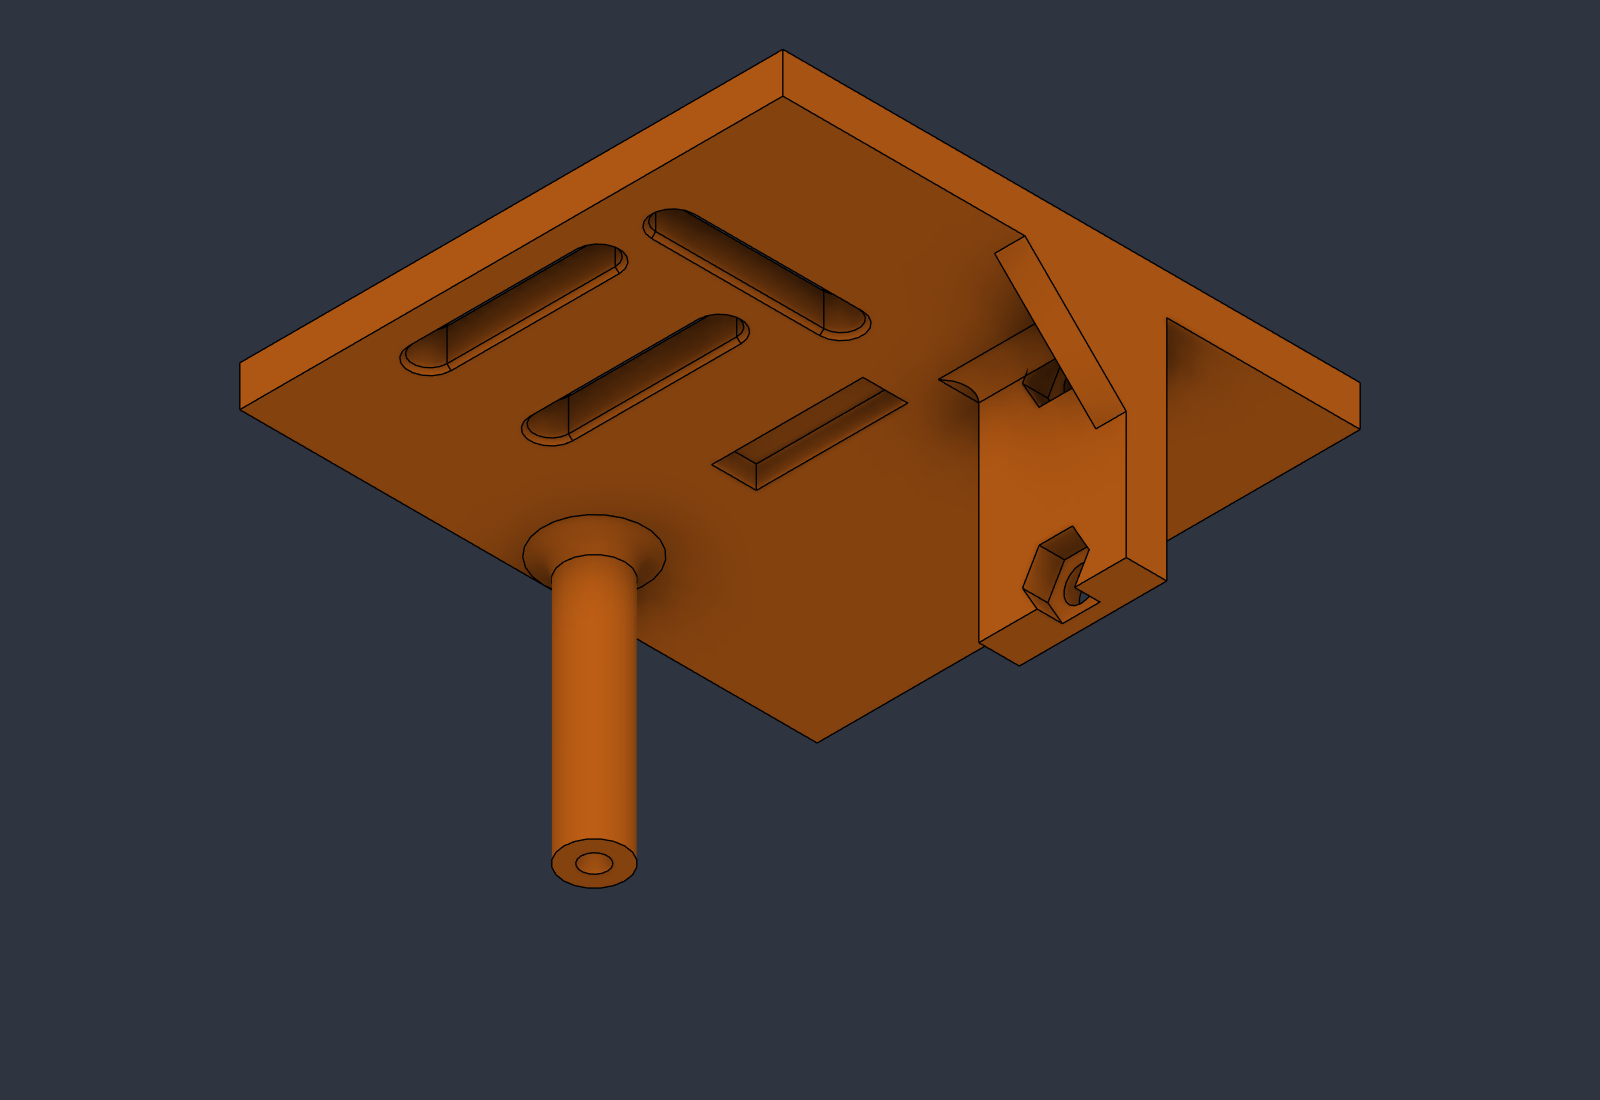
\includegraphics[width=0.48\textwidth]{angle_bracket_under_rear.png}
  \caption{Right bracket on its own: top and underside, from the front and the rear.}
  \label{fig:bracket-angles}
\end{figure}

% F11-F12 -- bracket with motor, disc and LM393 (no wheel, no plate), from below
\begin{figure}[htbp]
  \centering
  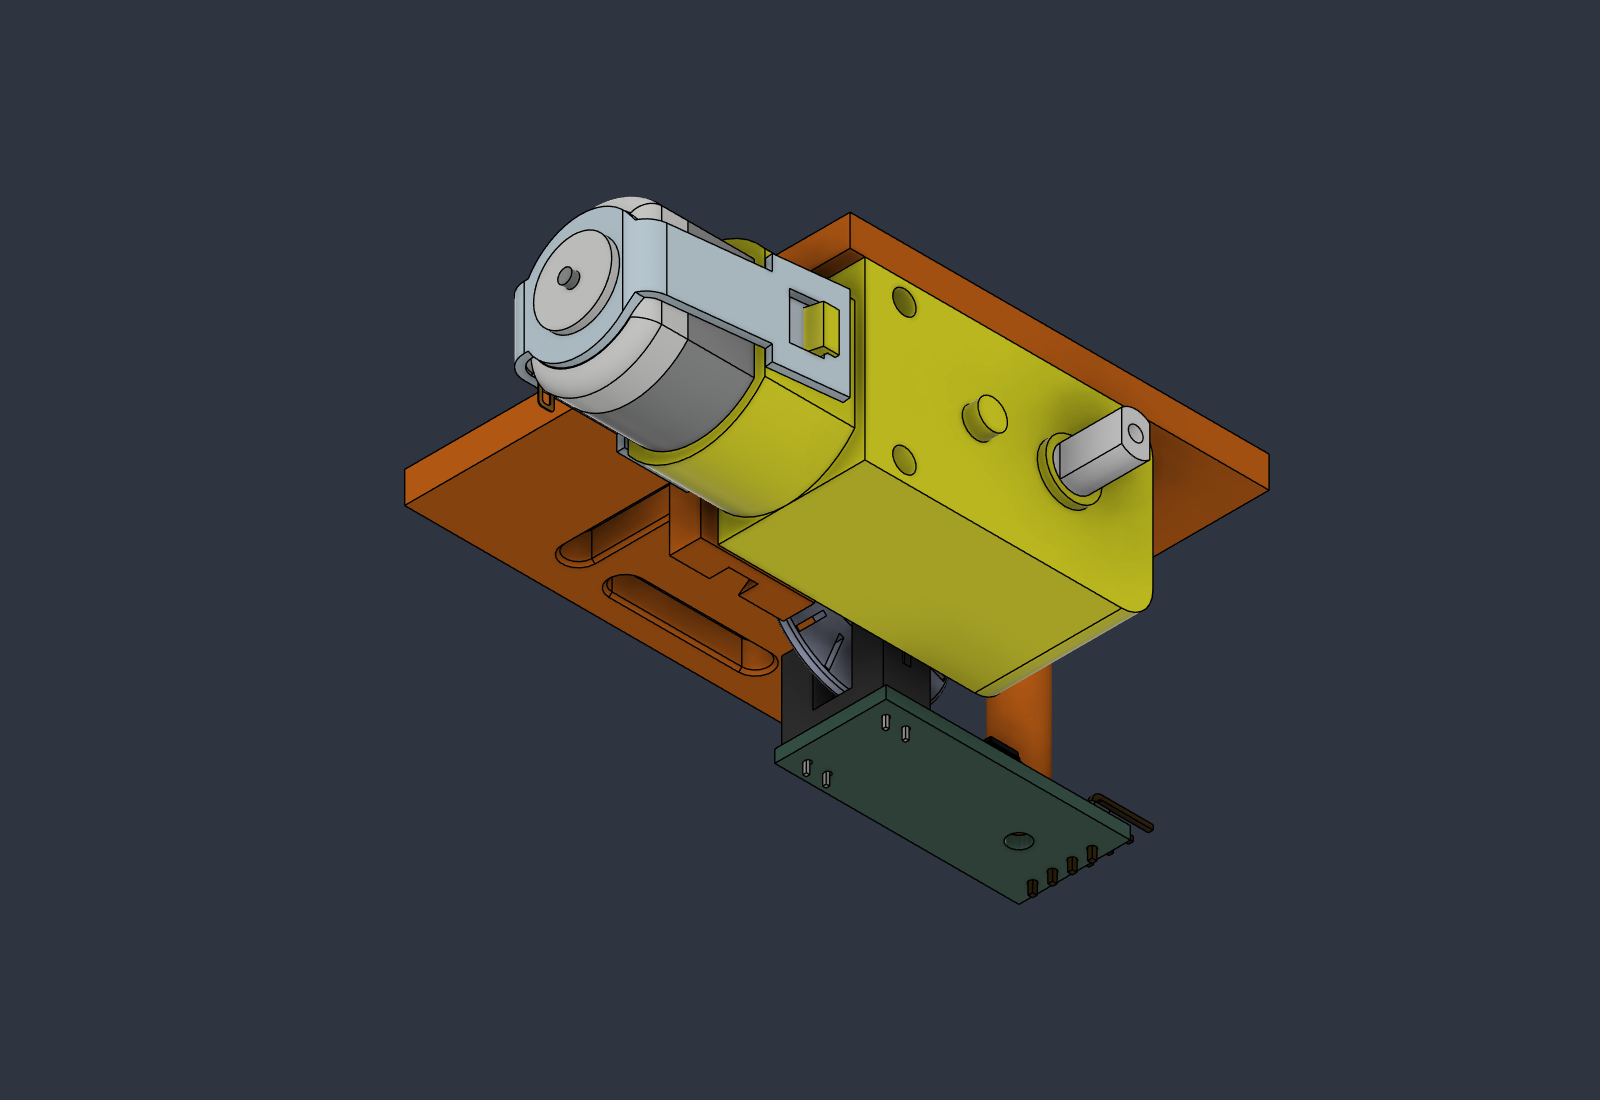
\includegraphics[width=0.48\textwidth]{angle_assembly_under_front.png}\hfill
  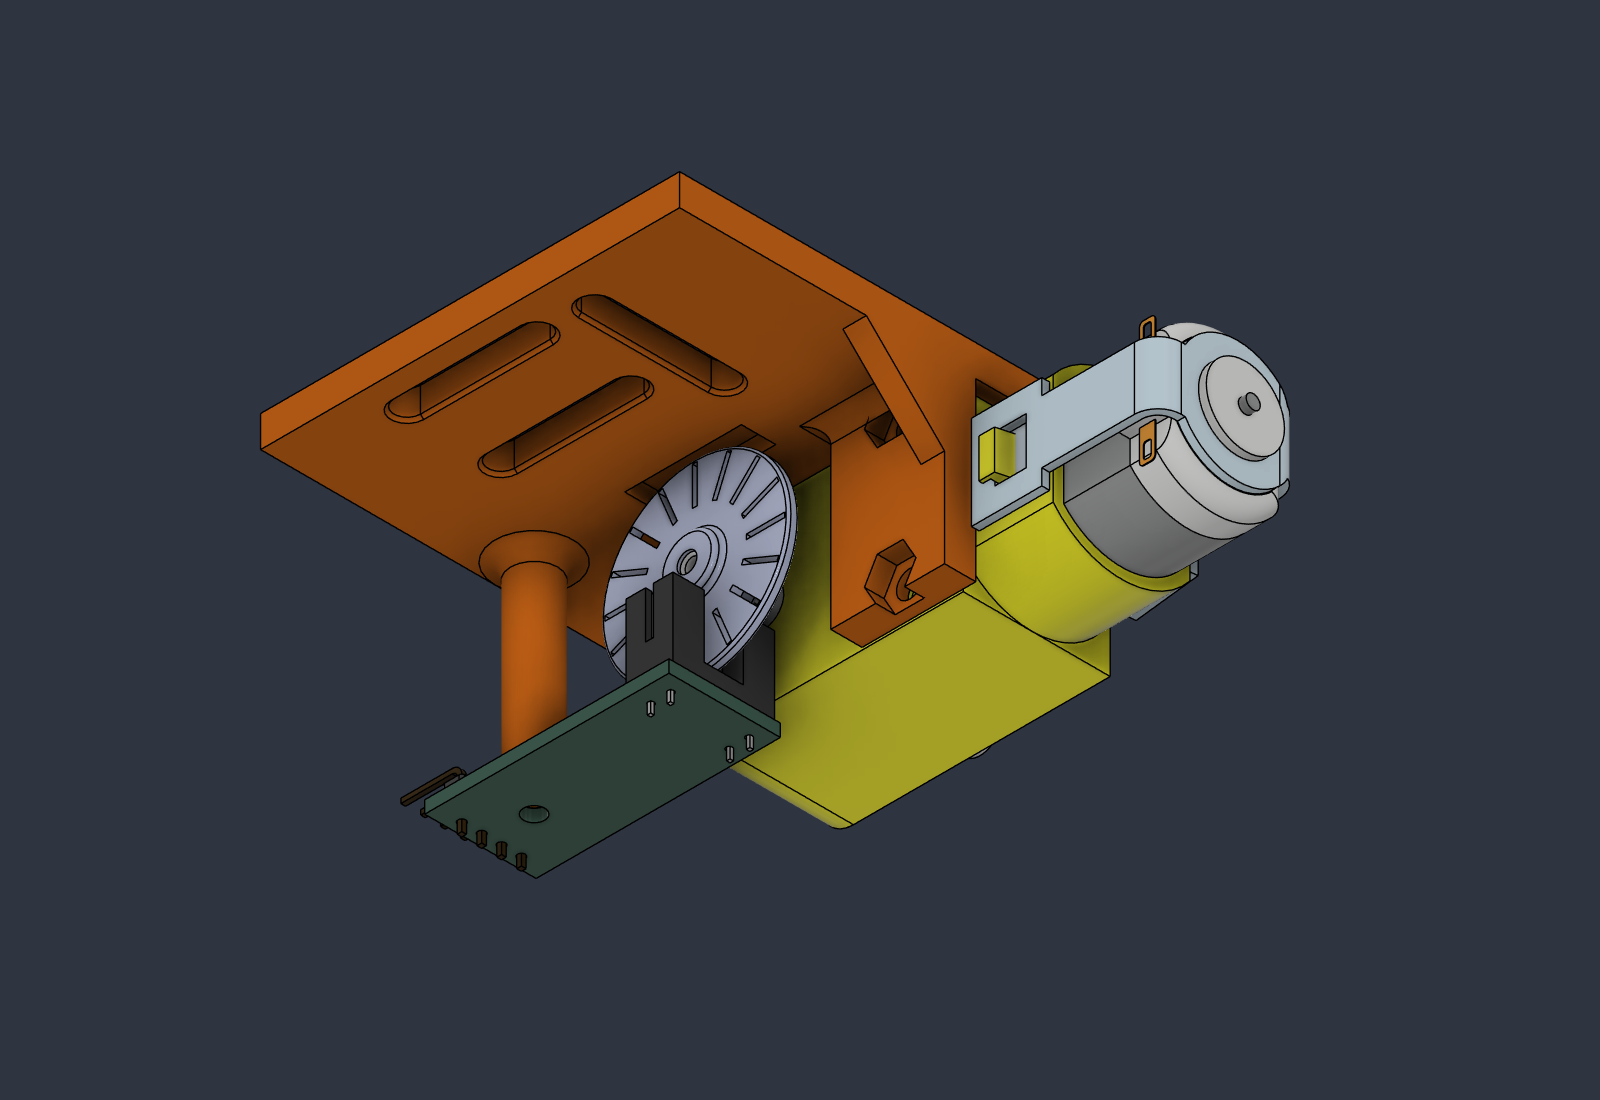
\includegraphics[width=0.48\textwidth]{angle_assembly_under_rear.png}
  \caption{Assembly from below: motor tab and nut traps, encoder disc and LM393 sensor.}
  \label{fig:assembly-below}
\end{figure}


\printbibliography
\end{document}
